% !Mode:: "TeX:UTF-8"
% vim: set foldmethod=marker sw=4 ts=4 noet:
\makeatletter
	\@namedef{ver@natbib}{opt@sort&compress}
\makeatother
\documentclass[bachelor,openany,oneside,color]{buaathesis}

% {{{ 导入宏包
\usepackage[backend=biber,style=gb7714-2015]{biblatex}
	\addbibresource[location=local]{QIN.bib}
\usepackage{tikz,amsmath,amssymb}% for common math symbols
	\usetikzlibrary{positioning,snakes}
%%\usepackage{gensymb}%other sumbles as \degree
\usepackage{booktabs}%for table \toprule and \bottomrule
\usepackage{physics}
\usepackage{bm}%for \bm{vector}
\usepackage{braket}%for \bra and \ket
%\usepackage{mathtools}%for correct \sum
\usepackage{commath}%for \abs
%\usepackage{mhchem} %for chemistry symbol \cm
\usepackage{mathrsfs}%for \mathscr characters
\usepackage{chngcntr,hyperref}%for hyperlink of reference
\usepackage{url}
	\PassOptionsToPackage{hyphens}{url}
\usepackage{cleveref}
\usepackage{etoolbox}%for \ifcsdef
\usepackage{siunitx}%for units
	\DeclareSIUnit\year{a}
	\DeclareSIUnit\gauss{Gs}
\usepackage{subcaption}
\def\TZ{T\textsubscript{0}}
\def\PrimaryParticle{\textsuperscript{12}C}

%\usepackage[top=1in, bottom=1in, left=1.25in, right=1.25in]{geometry}% page size
%\usepackage[font=small,width=0.8\textwidth,labelfont=bf]{caption}%for caption font
%\usepackage{subcaption} %for \subcaption{} for {subfigure}
%\usepackage{longtable}%for longer tables
%\usepackage{multirow}%for combined rows
%\usepackage{changepage}%for displaying page number
%\usepackage{fancyhdr}
%	\pagestyle{fancy}
%	\fancyhead{}
%	\fancyhead[RO,LE]{\thepage}
%	\fancyhead[LO,RE]{\SUBTITLE}
%	\fancyfoot{}
%	\renewcommand{\headrulewidth}{0pt}
%	\renewcommand{\footrulewidth}{0pt}

%\usepackage{autobreak,breqn}

%%=== ntheorem ===
%\usepackage[amsmath,thmmarks]{ntheorem}% for {theorem}
%	\theoremstyle{plain}
%	\theoremheaderfont{\normalfont\rmfamily\CJKfamily{hei}}
%	\theorembodyfont{\normalfont\rm\CJKfamily{kai}}
%	\theoremindent0em
%	\theoremseparator{\hspace{1em}}
%	\theoremnumbering{arabic}
%	\theoremsymbol{■}          %symbol added after end of theorem
%	\newtheorem{theorem}{Theorem}[subsection]
%	\newtheorem{defn}{Definition}[subsection]

%%=== lstlisting ===
%\usepackage{listings,color}
%	\definecolor{mygreen}{rgb}{0,0.6,0}
%	\definecolor{mygray}{rgb}{0.9,0.9,0.9}
%	\definecolor{mymauve}{rgb}{0.58,0,0.82}
	\lstset{ %
%	  backgroundcolor=\color{mygray},   % choose the background color; you must add \usepackage{color} or \usepackage{xcolor}; should come as last argument
	  basicstyle=\footnotesize,        % the size of the fonts that are used for the code
%	  breakatwhitespace=false,         % sets if automatic breaks should only happen at whitespace
%	  breaklines=true,                 % sets automatic line breaking
%	  captionpos=b,                    % sets the caption-position to bottom
%	  commentstyle=\color{mygreen},    % comment style
%	  deletekeywords={...},            % if you want to delete keywords from the given language
%	  escapeinside={\%*}{*)},          % if you want to add LaTeX within your code
%	  extendedchars=true,              % lets you use non-ASCII characters; for 8-bits encodings only, does not work with UTF-8
%	  frame=single,	                   % adds a frame around the code
%	  keepspaces=true,                 % keeps spaces in text, useful for keeping indentation of code (possibly needs columns=flexible)
%	  keywordstyle=\color{blue},       % keyword style
%	  language=Mathematica,                 % the language of the code
%	  morekeywords={*,...},           % if you want to add more keywords to the set
%	  numbers=left,                    % where to put the line-numbers; possible values are (none, left, right)
%	  numbersep=5pt,                   % how far the line-numbers are from the code
%	  numberstyle=\tiny\color{mygray}, % the style that is used for the line-numbers
%	  rulecolor=\color{black},         % if not set, the frame-color may be changed on line-breaks within not-black text (e.g. comments (green here))
%	  showspaces=false,                % show spaces everywhere adding particular underscores; it overrides 'showstringspaces'
%	  showstringspaces=false,          % underline spaces within strings only
%	  showtabs=false,                  % show tabs within strings adding particular underscores
%	  stepnumber=1,                    % the step between two line-numbers. If it's 1, each line will be numbered
%	  stringstyle=\color{mymauve},     % string literal style
%	  tabsize=2,	                   % sets default tabsize to 2 spaces
%	  title=\lstname                   % show the filename of files included with \lstinputlisting; also try caption instead of title
	}

%% define math operators
\def\D{\mathrm{d}}
\def\Ln{\mathrm{ln}}
\def\CH{\mathrm{CH}}
\def\FWHM{\mathrm{FWHM}}
\def\figureinit{\centering\setlength\parindent{0pt}}
% }}}

\begin{document}

% {{{ 前缀部分
% 用户信息
% !Mode:: "TeX:UTF-8"

% 学院中英文名,中文不需要“学院”二字
% 院系英文名可从以下导航页面进入各个学院的主页查看
% http://www.buaa.edu.cn/xyykc/index.htm
\school
{物理科学与核能工程}{School of Physics and Nuclear Energy Engineering}

% 专业中英文名
\major
{核物理}{Nuclear Physics}

% 论文中英文标题
\thesistitle
{HIRFL-CSR外靶实验终端模拟和分析框架的构建}
{}
{Establishment of a terminal simulation and analyzation framework for
 HIRFL-CSR External Target Experiment (CEE)}
{}

% 作者中英文名
\thesisauthor
{秦雨浩}{QIN Yuhao}

% 导师中英文名
\teacher
{肖志刚}{Zhigang XIAO}
% 副导师中英文名
% 注:慎用‘副导师’,见北航研究生毕业论文规范
%\subteacher{副导师}{subteacher}

% 中图分类号,可在 http://www.ztflh.com/ 查询
\category{TP312}

% 本科生为毕设开始时间;研究生为学习开始时间
\thesisbegin{2018}{01}{01}

% 本科生为毕设结束时间;研究生为学习结束时间
\thesisend{2018}{06}{01}

% 毕设答辩时间
\defense{2018}{06}{01}

% 中文摘要关键字
\ckeyword{外靶实验,探测器构建,框架,数字化}

% 英文摘要关键字
\ekeyword{external target experiment, detector construction, framework, digitize}

\makeatletter
\hypersetup{
	pdftitle={\buaa@thesistitle},
	pdfauthor={\buaa@thesisauthor}
}
\makeatother
% !Mode:: "TeX:UTF-8"

% 班级
\class{141913}

% 学号
\studentID{14191033}

% 单位代码
\unicode{}

% 论文时间,用于首页
\thesisdate{2018}{06}


% 任务书信息
% !Mode:: "TeX:UTF-8"
% 任务书中的信息
%% 原始资料及设计要求
\assignReq
{\textbf{CSR外靶实验(CEE)}:利用中国科学院近代物理研究所的重离子加速器}
{提供的束流进行的重离子 碰撞外靶实验。现已立项低温高密度核物质测}
{量谱仪,即为本框架要求构建的探测器阵列。[1]}
{\textbf{终端模拟和分析框架}:构建一套软件框架,对探测器进行构建、模拟和}
{数字化(digitization) 并提供可视化等分析功能。[2][3]}
%% 工作内容
\assignWork
{构建框架至少应当完成以下工作:}
{1. 构建探测器,对每种探测器构建其几何模型与数字化模型;}
{2. 构建针对HIRFL-CSR外靶实验的粒子源和物理过程列表;}
{3. 基于外靶实验设计构建电磁场环境;}
{4. 调用框架实现对CEE实验的模拟、数字化与分析;}
{5. 利用有关框架实现可视化等分析功能。}
%% 参考文献
\assignRef
{[1] CEE 合作组.CEE 技术文档 1[R].2017.10}
{[2] GSI. About FairRoot[EB/OL]. https://fairroot.gsi.de/?q=about}
{[3] CERN. Geant4 User's Guide for Application Developers 10.3[M], 2016-12-06}
{}
{}
{}
{}
{}


% 页眉页脚样式
\pagestyle{mainmatter}
% 封面、任务书、声明
\maketitle
% 摘要
% !Mode:: "TeX:UTF-8"

% 中英文摘要
\begin{cabstract}
本篇文章主要介绍一套用于HIRFL-CSR外靶实验(CEE)模拟与分析的软件框架。本文首先介绍
了CEE实验的概况和主要涉及的探测器原理与布置,之后介绍了本软件框架的基本原理、主要
结构与关键技术难点的实现方法,最后给出了探测器模拟的一组结果和分析方法。
\end{cabstract}

\begin{eabstract}
A simulation and analyzation software framework for HIRFL-CSR External Target
Experiment (CEE) is built and introduced. Goals and detectors of CEE experiment are
reviewed as an introduction. Basic principles, main structure and implementations
for certain technological problems are introduced. A group of simulation results and
routes of analyzation are given as a conclusion.
\end{eabstract}

% 目录
\tableofcontents

% 正文页码样式
\mainmatter
% }}}

%% 正文
\chapter{绪论}
% {{{ 绪论 

\section{课题背景}

在中高能粒子物理的实验研究中,对实验环境和探测器响应的模拟是实验准备阶段的一大核心
工作。根据这些模拟的结果,可以在实验准备阶段确定实验对不同探测器的性能提出的要求,
以评价和调整实验方案。目前,对粒子物理的模拟研究主要基于Geant4模拟框架。该框架是一
套C++软件框架,提供了一套根据给定的物理过程列表追踪粒子及其次级粒子的工具。用户需要
使用C++语言编写或重载有关的类,以构建探测器、其数字化模块和场等其他环境因素。这种形
式意味着需要针对每个模拟问题构建一个新的模拟应用程序,并设计其数字化和数据存储与处
理的有关功能。

\section{国内外研究现状}

%%CEE
\subsection{CSR外靶实验(CEE)}

本研究所称的“HIRFL-CSR外靶实验”,指的是利用中科院近代物理研究所的重离子加速器提供的
束流进行重离子碰撞外靶实验(CSR External-target Experiment,CEE)。

该实验已经立项搭建低温高密核物质测量谱仪。该谱仪的测量手段为,利用大接收度的超导磁铁
,通过时间投影室、硅像素、高计数率飞行时间谱仪等多种国内首次采用的先进探测器,配合先
进的电子学技术,实现对中能重离子碰撞产物的全空间探测和鉴别。本研究的主要内容就是基于
CEE的设计构建软件层面的终端模拟和分析框架。

该实验将构建低温高密核物质测量谱仪,通过相对论重离子碰撞实验实现QCD相变。国际上已经
有多个类似的重离子碰撞实验,但基本运行在高能区。
\begin{itemize}
	\item 美国的相对论重离子对撞机(RHIC),每对核子对撞能量达\SI{200}{\giga\eV};
	\item 欧洲核子中心的大型强子对撞机(LHC),能量可达\SI{5.4}{\tera\eV},以寻找
		高温夸克胶子等离子体并探索其性质;
	\item 德国的反质子-离子研究装置(FAIR)上将要运行的压缩强子物质实验(CBM),
		每核子能量达\SI{45}{\giga\eV},主要目的是探索高密QCD相变和临界点。
\end{itemize}
国际上已有的重离子碰撞实验鲜有涉及低温而更高重子化学势(重子数密度)的区域,这一区
域恰好是HIRFL-CSR和将来HIAF装置将覆盖的区域。RIEFL-CSR能够提供$0.5\sim\SI{1.2}
	{\giga\eV}$的离子束流,QCD相图在这一区域有非常丰富的结构和与恒星演化密切相关的
状态方程信息。

%%GSI
\subsection{终端模拟和分析框架}

终端模拟和分析框架指的是构建一套软件框架,对探测器进行构建、模拟和数字化(digitize,
指将模拟中探测器灵敏的物理量转换为读出系统的实际输出)。核物理与高能物理领域内常用到
模拟框架Geant4与分析框架ROOT。Geant4需要为每个模拟问题专门编写程序,构建探测器并存
储所需的物理信息;ROOT主要用于对数据的统计分析。

以上述德国的FAIR装置为例,GSI开发了一套面向对象的模拟、重建和数据分析框架FairRoot。
该框架下可以将每个探测器构建为由数字化参数构建、几何参数构建、蒙特卡洛模拟等若干个
类组成的类库,还可以实现粒子轨迹的可视化等针对整个外靶实验的功能。\cite{FairRoot}
FAIR上正在筹备的CBM实验基于该框架构建了数据分析软件CbmRoot,其中构建了其中用到的
各探测器及其布局,能够对整个实验进行模拟、重建和事件显示等。

\section{课题目的}

本研究的主要目的是基于HIRFL-CSR外靶实验的设计和实际情况,构建终端模拟和分析框架。
经过调研,构建框架至少需要完成以下的工作。
\begin{enumerate}
	\item 构建探测器:对每种类型的探测器都至少需要完成以下工作:
	\begin{enumerate}
		\item 读取探测器的几何参数,构建探测器的几何形态;
		\item 读取和构建探测器的材料信息;
		\item 设计各种探测器的数字化模块,基于探测器的工作原理给出读出系统的输出;
	\end{enumerate}
		以实现对探测器主要功能的模拟。
	\item 基于HIRFL-CSR的实际情况,构建粒子源和物理列表;
	\item 基于外靶实验的设计,构建实验环境的电磁场等因素;
	\item 调用以上构建出来的框架,实现对整个实验的模拟、数字化和重建等功能;
	\item 调用分析框架提供的显示功能,实现对事件进行可视化的功能。
\end{enumerate}

\section{论文构成及研究过程}

\subsection{论文构成}

本论文将主要围绕CEE实验概况、模拟框架的主体结构、关键技术难点的实现和模拟样例与分析
四部分展开。其中,实验概况将介绍CEE实验的物理目标、计划选用的探测器类型与功能,以及
实验的探测器布局等信息,以作为本文的构建基础;主体结构将介绍本框架所划分的主要模块及
其功能;关键技术难点将介绍MRPC、TPC和MWDC三种探测器的数字化实现原理,以及径迹重建的
基本原理。

\subsection{研究过程}

本研究主要围绕Geant4框架的学习和对探测器原理的学习逐渐展开,工作过程大致可以分为以
下的几个阶段。
\begin{enumerate}
	\item 1--2月:调研模拟框架的原理,学习基础知识;
	\item 3月:实现简单的几何构建,实现粒子源、物理列表和材料构建;
	\item 4月:完成几何构建,实现简单的数字化模块;
	\item 5月:实现关键探测器的数字化功能,分析输出结果。
\end{enumerate}

实际开展工作的过程中,在调研阶段形成了基于GSI的FairRoot框架或直接基于Geant4框架
编写的两个路线。由于FairRoot和CbmRoot的文档严重不足,而Geant4有比较完善的手册
\cite{Geant4},本工作选择了基于Geant4开发框架。在4月的中期检查前,本框架完成了
主要几何构建,实现了能量沉积、起始时间等简单的数字化模块;之后的一个月内完成了
本文将在第\ref{chap:digi}中重点讨论的较复杂的数字化工作。
% }}}

\chapter{CEE实验概况}
% {{{ CEE实验概况 

本框架的设计目标是对CEE的探测器系统进行构建和模拟,并准备用于CEE实验的分析;本章将
介绍CEE实验的主要物理目标、需要在框架内给出构建的主要子系统,以及整个探测器系统的
概览图。

\section{物理目标}

CSR外靶实验(CEE)的探测器系统被称作“低温高密核物质测量谱仪”,这一谱仪将是我国
第一台运行于\si{\giga\eV}能区的、完全自主研制的、基于国内核物理大科学装置
HIRFL-CSR的大型核物理实验装置。其主要的科学功能是实现该能区的重离子碰撞中带电粒子
产物的近全空间测量,为致密天体性质、核反应动力学、自旋和同位旋相关的核力与
核物质状态方程性质、高重子数密度QCD相图等重要的科学问题研究提供基础实验数据。
\cite{技术文档,Lyu:ConceptDesign}

\section{主要子系统}

CEE的主要子系统包括磁场、探测器系统、读出系统与靶。其中,探测器系统主要包括
微像素定位探测器、径迹探测器、飞行时间探测器(TOF)和零度角量能器(ZDC)这四类。
本节将介绍磁场系统,以及各类探测器的用途、原理和CEE中采用探测器的设计要点。

\subsection{磁场系统}

CEE的磁场系统主要是一个由超导二极磁铁产生的在
$\SI{1}{\meter}\times\SI{0.9}{\meter}\times\SI{1.2}{\meter}$(长、高、宽)
的大范围内保持高均匀度的磁场,中心区域场强控制为\SI{0.5}{\tesla}。
该磁场的主要功能是偏转带电粒子,使带电粒子在磁场内的径迹探测器中产生偏转径迹,利用
探测到的重建径迹得到粒子的动量。最简单的情况是对非相对论粒子(如重离子),忽略粒子
穿过探测器通过电离等形式发生的能量损失、忽略竖直方向电场等作用的情况,并假定磁场
方向与运动平面垂直时,可以认为其所受的洛伦兹力$\bm{F}$提供偏转向心力:
\begin{equation}\label{eq:B}
\bm{F} = -\frac{mv^2}{R}\hat{\bm{n}} = q\bm{v}\times\bm{B}
\end{equation}
其中$m$为粒子质量,$\bm{v}$为速度,$R$为偏转半径,$\hat{\bm{n}}$为径向单位矢量,
$\bm{B}$为磁场的磁感应强度;于是有
\begin{equation}
p = q B R
\end{equation}
其中$p$为粒子动量大小。因此,在重建得到半径的情况下,可以确定已知电荷量粒子的动量。

CEE所用的磁场本质上是服务于径迹探测器中的时间投影室探测器(Time Projection Chamber,
TPC)的,因此其可以被简化为覆盖一个包覆了TPC探测器的固定尺寸的长方体范围的
局域匀强磁场。

\subsection{微像素定位探测器}\label{ssec:det:track}

微像素定位探测器(Pix)主要用于提供束流的入射方向以及对发生反应的顶点位置进行精密
测量。这一探测器本质上是一只无磁场的充有Ar/CO\textsubscript{2}$70:30$工作气体的
漂移室,电子漂移约3-\SI{5}{\centi\meter},到达读出阳极前由气体电子倍增器
(Gas Electron Multiplier,GEM)进行一次放大;读出端为二维微像素传感器TopModel,
可以读出漂移电子在读出端平面上的位置投影。Pix探测器的结构如图\ref{fig:det:Pix}所示。

\begin{figure}
	\centering
	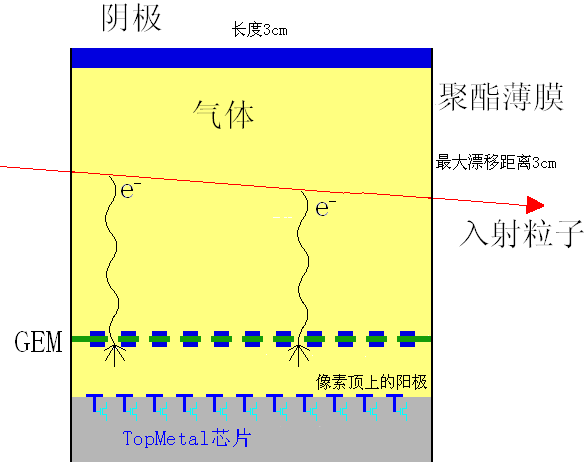
\includegraphics[width=0.5\textwidth]{./resource/CEE-Pix.png}
	\caption{微像素定位探测器的原理示意图}
	\label{fig:det:Pix}
\end{figure}

Pix探测器的主要作用是确定入射粒子的初始位置。对于模拟框架而言,这一探测器的功能
可以由对粒子源参数的控制实现。

\subsection{径迹探测器}

径迹探测器的主要用途是获取粒子径迹,从而得到粒子动量和进行粒子甄别。CEE实验中采用
的径迹探测器主要有时间投影室(Time Projection Chamber, TPC)和
多丝漂移室(MWDC);它们分别覆盖束流的正方向的大角度区和偏离束流方向的小角度区。

\subsubsection{时间投影室(TPC)}

TPC探测器的主要原理是在气体漂移室探测器中加以匀强电场,使入射粒子在灵敏区内产生的
带电次级粒子受到的电场力与气体内的阻力平衡,从而使次级粒子沿电场方向做匀速运动,
以将粒子在电场方向的径迹位置投影为漂移时间;在垂直电场方向的阳极面上设置空间灵敏的
气体电子倍增器(Gas Electron Multiplier, GEM)雪崩放大及感应阵列探测次级粒子
(时间信息来自漂移速度快的电子),从而得到垂直电场方向的位置投影信息。一般为了简化
探测器结构,磁场和电场在同一方向上。
例如,假设次级粒子在漂移室内运动所受阻力为
$\bm{F}_\nu=-\alpha\bm{v}$($\alpha$为阻力系数,$\bm{v}$为粒子速度),平衡状态下
粒子运动方向应当与电场方向平行,并满足电场力与阻力平衡:
\begin{equation}\label{eq:det:other:eq}
	\bm{F}_\nu+q\bm{E}=-\alpha\bm{v}+q\bm{E}=0
\end{equation}
其中$q$为次级粒子所带电荷;$\bm{E}$为TPC内的匀强电场。因此,对于一定的粒子(具有
确定的阻力系数和电荷量),其漂移速度是一个定值。电子事实上并不满足上式,但电子同样
可以做匀速漂移;例如,某条件下电子在气体中的漂移速度如图\ref{fig:Drift}所示。

\begin{figure}\centering
	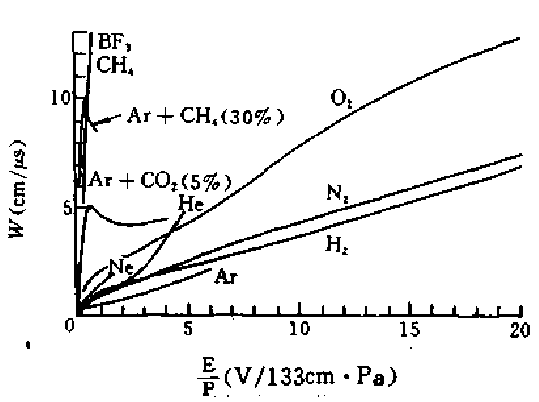
\includegraphics[width=0.4\textwidth]{./resource/Electron-Drift-Speed.png}
	\caption{电子在气体中的漂移速度\cite{核物理实验方法:气体}}
	\label{fig:Drift}
\end{figure}

在次级粒子中,电子的漂移速度远大于离子,而复合概率则远小于离子,因此TPC中感应到的
信号主要为漂移电子。电子开始加速后,能量逐渐增大,超过工作气体的激发能级时开始引发
大量能量损失的非弹性碰撞,最终能损等于电子从电场获得的能量而达到平衡,从而得到恒定
的漂移速度。\cite{核物理实验方法:气体}
%电子的平均能量为:
%\begin{equation}\label{eq:det:electron:eq}
%\frac12 m u_e^2 = \ita \frac32 k T
%\end{equation}
%式中$u_e$为电子的杂乱运动速度,$\frac32kT$为平衡热运动能量,$k$为玻尔兹曼常数,$T$
%为气体的绝对温度,$\ita$为电子的温度。
在CEE所采用的TPC中,漂移速度为\SI{5}{\centi\meter/\micro\second}。

本质上,TPC探测器可以视为一个主要对电子时间和位置灵敏的探测器;应当可以读出粒子在
TPC中划过径迹的位置,在垂直于电场的方向上划分为若干灵敏块(按照各个读出单元的
灵敏范围),并记录每个灵敏块的能量沉积漂移时间。

实验上TPC中不同位置对应的读出单元、漂移时间等均需要通过实验精确刻度。按照CEE的设计,
预备使用能使TPC工作气体电离的高能脉冲激光系统完成对电子的漂移时间、电场的质量以及
磁场的均匀度等问题的标定。

\subsubsection{多丝漂移室(MWDC)}

CEE中采用的多丝漂移室系统由六块MWDC组成,分别配置在上述磁铁下游方向的束流线两侧,
每侧分别平行放置三块;每块MWDC由三层成角度的灵敏丝层组成。当粒子穿过MWDC时,在
每块MWDC内可以在三层灵敏丝上分别产生打火信号,从而确定穿过点的位置并评判其可信度。

每块MWDC包含三层灵敏丝,分别记作X、U和V丝,其灵敏丝与竖直方向分别成
\SI{0}{\degree}、\SI{30}{\degree}和\SI{-30}{\degree}角,如图\ref{fig:det:MWDC}
所示。每层丝并没有做双层读出,而是利用三层加上三块平行MWDC得到的九层灵敏丝来拟合
径迹。作为漂移室,入射粒子在MWDC的灵敏层产生次级粒子后,可以利用次级粒子的漂移时间
得到更精确的位置;其起始时间可以由放置在三组MWDC后的外部飞行时间探测器eTOF给出。

\begin{figure}
	\centering
	\begin{subfigure}{0.4\textwidth}
		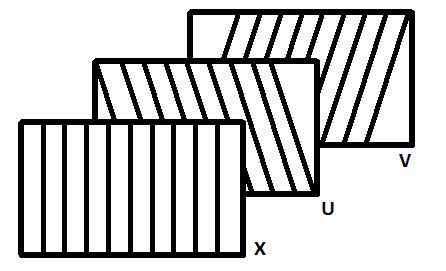
\includegraphics[width=\textwidth]{./resource/CEE-MWDC-Layer.jpg}
		\subcaption{MWDC的阳极丝几何角度示意图\cite{技术文档}}
		\label{fig:det:MWDC:Layer}
	\end{subfigure}
	\begin{subfigure}{0.4\textwidth}
		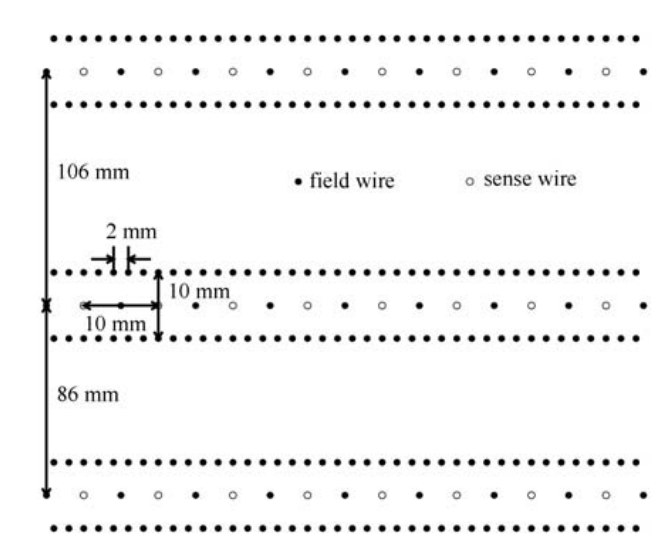
\includegraphics[width=\textwidth]{./resource/CEE-MWDC-Layout.png}
		\subcaption{MWDC的结构,未按比例,每层均旋转到X层的方向\cite{Yi:MWDC}}
		\label{fig:det:MWDC:Layout}
	\end{subfigure}
	\caption{MWDC的结构示意图}\label{fig:det:MWDC}
\end{figure}

这一MWDC系统可以抽象为一个空间灵敏探测器,每块探测器可以分为三层,在每层能够记录
打火信号的一维位置信息,以及漂移时间的信息;在精确标定后,可以通过漂移时间确定
漂移距离;利用多层丝的符合,可以精确测量粒子穿过MWDC的位置信息;利用三块探测器
的符合,可以确定粒子在MWDC系统内的径迹,从而确定粒子的动量和角度信息。事实上,
CEE中采用MWDC的主要作用就是提供高质量的角度关联信息。

\subsection{飞行时间探测器}

CEE实验拟采用的飞行时间探测器均为多气隙电阻板室(MRPC)阵列,主要包括磁场外部、
束流线下游的端盖飞行时间探测器(eTOF),磁铁轭铁与TPC之间的内部飞行时间探测器
(iTOF)和起始时间探测器(\TZ)。

这些飞行时间探测器的本质均为多层MRPC阵列。CEE采用的MRPC阵列的最基本单元是条状的
MRPC小室,每个小室内充有工作气体,由若干层普通玻璃或低电阻玻璃分割成若干个气隙;
中间设置焊有若干金属条的读出条,能够从两端读出并通过信号时间差确定位置信息。
MRPC的结构图如图\ref{fig:det:TOF:MRPC}所示。

为尽可能减少死区,组成飞行时间探测器的MRPC交错布置,组成一堵“TOF墙”;例如,
端盖飞行时间探测器(eTOF)的概念性设计如图\ref{fig:det:TOF:eTOF}所示。

\begin{figure}
	\centering
	\begin{subfigure}{0.3\textwidth}
		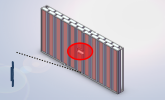
\includegraphics[width=\textwidth]{./resource/CEE-eTOF.png}
		\subcaption{端盖飞行时间探测器(eTOF)的概念性设计}
		\label{fig:det:TOF:eTOF}
	\end{subfigure}
	\begin{subfigure}{0.5\textwidth}
		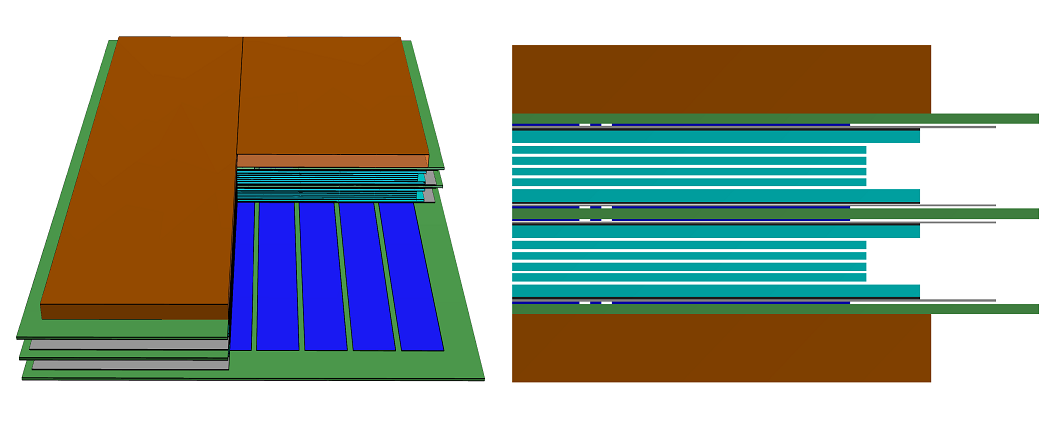
\includegraphics[width=\textwidth]{./resource/CEE-MRPC.png}
		\subcaption{条形读出MRPC的结构图}
		\label{fig:det:TOF:MRPC}
	\end{subfigure}
	\begin{subfigure}{0.5\textwidth}
		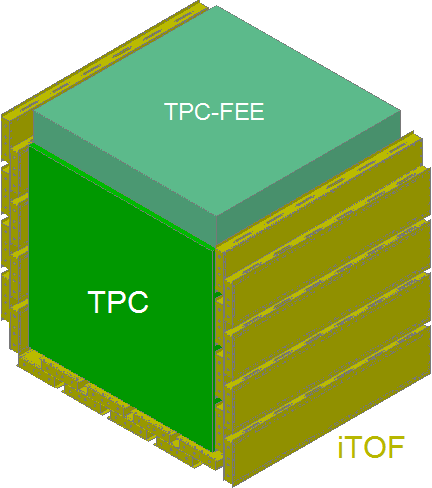
\includegraphics[width=\textwidth]{./resource/CEE-iTOF.png}
		\subcaption{内部飞行时间探测器(iTOF)的配置}
		\label{fig:det:TOF:iTOF}
	\end{subfigure}
	\caption{飞行时间探测器的设计\cite{技术文档}}
	\label{fig:det:TOF}
\end{figure}

端盖飞行时间探测器(eTOF)设置在磁场外部、束流线下游,主要用途是鉴别(通过
MWDC的)带电粒子种类。内部飞行时间探测器(iTOF)设置在磁场的轭铁与中央的
TPC的外表面之间,用于有效鉴别末态粒子,其配置如图\ref{fig:det:TOF:iTOF}所示。

CEE所采用的各种TOF均可以抽象为对时间和位置灵敏的探测器,
可以为每组输出起始时间、横向的位置信息(金属条的编号)和
信号到达两端的时间差(反映一维位置信息)。

\subsection{零度角量能器(ZDC)}

ZDC位于探测器系统的最后,可以接收到受磁场偏转影响较小的强子。该量能器的基本结构
为铅和闪烁体夹层,可以读出事件沉积的总能量。

CEE采用的ZDC的基本结构为65层铅与65层闪烁体交叉放置的量能器,面向入射粒子流角度
方向。其测量出的总能量被用于做中心快度关联函数测量等。CEE采用的ZDC的设置图如
图\ref{fig:det:ZDC}所示。

\begin{figure}
	\centering
	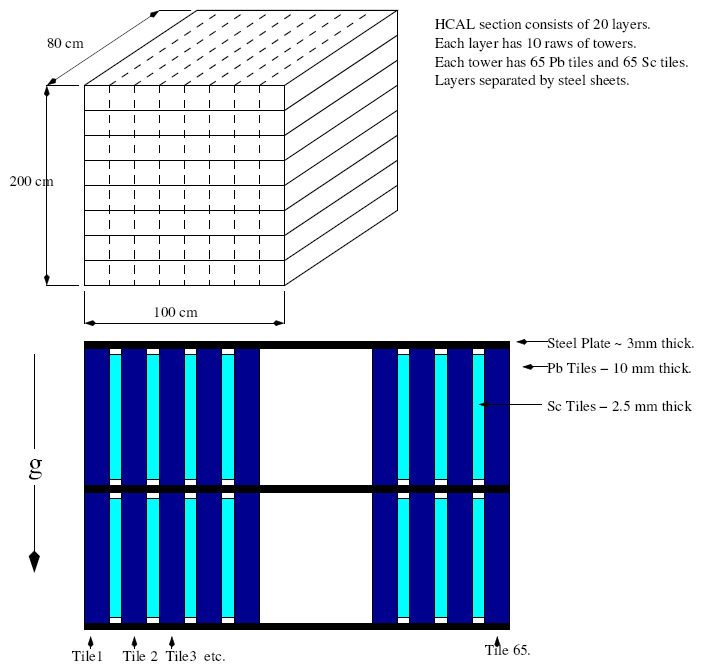
\includegraphics[width=0.6\textwidth]{./resource/CEE-ZDC.png}
	\caption{CEE的ZDC系统设图\cite{技术文档}}
	\label{fig:det:ZDC}
\end{figure}

\section{实验布局}

CEE拟利用粒子在磁场中的偏转,通过测量粒子的径迹和飞行时间实现对粒子动量的重建
和种类鉴别。\cite{技术文档,Lyu:ConceptDesign}CEE谱仪的核心部件为大接收度的二极磁铁与置于磁场内的
实现三维测量的TPC;为处理束流附近的死区,磁场下游方向束流两侧布置有两组MWDC
阵列;为实现轻粒子甄别,在TPC外和MWDC后设置有以MRPC阵列组成的飞行时间探测器
(TOF)和时间起始探测器\TZ;最后设置有零度角量能器ZDC。整体构型如图
\ref{fig:CEE:Subsystem}所示。

\begin{figure}\centering
	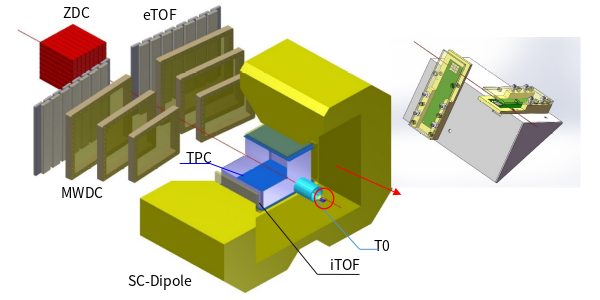
\includegraphics[width=0.9\textwidth]{./resource/CEE-Subsystem.png}
	\captionsetup{width=0.9\textwidth}
	\caption{CEE各子系统示意图。包括:SC-Dipole:超导二极磁铁;
		SiPiX:硅像素定位探测器;\TZ:起始时间探测器;TPC:中心时间投影室;
		iTOF:内飞行时间探测器;eTOF,端盖飞行时间探测器;
		MWDC:前角多丝漂移室径迹探测器;ZDC:零度角量能器
		\cite{技术文档,Lyu:ConceptDesign}}
	\label{fig:CEE:Subsystem}
\end{figure}

% }}}

\chapter{模拟框架的主体结构}
% {{{ 模拟框架的主体结构

本研究构建的模拟与分析框架目前主体是一个基于Geant4的C++应用程序,其中构建了所需的
探测器、与模拟有关的物理信息和数字化模块。其中,每个探测器都拥有自己的一套几何构建
与数字化模块,从而实现了每个探测器的模块化。

为了实现模拟,Geant4应用程序至少需要构建的功能主要包括探测器(以及其他环境几何体)
构建、主粒子生成(粒子源构建)和物理过程定义(物理列表)。\cite{Geant4}
为了将模拟结果转换为便于分析的格式,还需要利用分步操作等功能对模拟过程中的部分
物理量进行记录,以致转化为实验中电子学仪器的输出(这个过程称为数字化)。以下将分各
模块介绍本框架所采用的各个模块的基本结构与功能。

\section{几何构建}

Geant4中的探测器构建类主要需要提供Construct(几何构建)与ConstructSDandField(灵敏
探测器与场的构建)两个主要的虚函数。\cite{Geant4}本框架提供了这两个函数,分别用于
构建探测器几何结构与探测器的数字化功能。

几何构建方面,本框架为每一种探测器各提供了一个类,在类的构建函数中由外向内分别构建
了各种探测器的不同部分(如外壳、灵敏区等),最终给出整个探测器的逻辑体积(Logical
Volume)。这一过程中,构建函数将会从纯文本格式的数据文件中读取各个探测器组成部分
的尺寸信息。最终,探测器类将存有一个除了最终的摆放位置外全部构建完成的探测器,以及
从数据文件中读取的探测器摆放信息;该类最终在Construct函数中被实例化,并利用逻辑体积
和摆放位置生成其物理体积(Physical Volume)。各类还提供了一个函数GetSensitiveLVs,
返回所有灵敏区的逻辑体积列表,以方便数字化过程中判断粒子是否进入了灵敏区。

本框架内完成的几何构建有时间投影室探测器(TPC)、三种飞行时间探测器(TOF)、
多丝漂移室(MWDC)和零度角量能器(ZDC)。以下是每种探测器的主要构建方式。

\subsection{飞行时间探测器(TOF)}\label{ssec:det:tof}

本框架构建的飞行时间探测器主要有时间起始探测器(\TZ)、内部飞行时间探测器(iTOF)
和外部飞行时间探测器(eTOF)。本框架的几何构建中将这三种飞行时间探测器视为只有
层数、尺寸等参数差异的MRPC阵列,构建过程非常相似;但由于这三种探测器的参数差异
巨大,功能也有较大差异,因此本框架为三种探测器分别提供了自己的构建模块。

本框架中飞行时间探测器的构建主要分四层。第一层对应整个包装好的探测器,作为最外一层
,以及每个独立探测器的顶级对象;这部分可以对应探测器的外壳。第二层是探测器内的各个
子探测器单元,这些单元交错放置,以尽可能减小死区。第三层是每个单元内的MRPC单位,
这部分是TOF的主要灵敏区。第四层是MRPC单位内设置的多层玻璃板,其中也包括MRPC的
读出板,但本框架未构建读出板的PCB材料和上面划刻的金属条。其中,第三层的工作气体
被视为是整个探测器的灵敏体积:这部分扣除玻璃板等非灵敏区后,相当于MRPC的气隙。

最后,在探测器构建函数中,本框架将时间起始探测器\TZ 配置于整个探测器系统的最前方;
iTOF配置在TPC的两侧;eTOF配置在MWDC的后方。

所有探测器的参数都从格式相似的数据文件中读取。文件中的参数一直精确到每层玻璃的数据:
根据需要,可以对任何一块MRPC的参数特别配置参数,以及按照需要修改任何层级的单元的
个数。但整个TOF被视为确定个数的:本框架内只有一块\TZ、两块iTOF和两块eTOF,它们分别
拥有自己的一个数据文件。

\subsection{时间投影室探测器(TPC)}

本框架对TPC的几何构建相对简单。TPC的构建分为三层,第一层为用于确定位置的整体外壳,
第二层为腔室的外壳,第三层为腔室内的工作气体。三层均被构建为简单的长方体,由于GEM膜
、读出模块、金属条电场等附带的部分对主要粒子的运动影响有限,也为了提高模拟效率,
这些部分都没有进行几何构建。

这几层组件的编号和数据均从数据文件中读出。如果有需要,可以在数据中将TPC的几何结构
配置得更细致:例如将最内侧的工作气体腔设置成若干相切的小气腔等。为提高效率,目前
默认数据中每层均只有一个长方体,互相嵌套而得到整个TPC。

\subsection{多丝漂移室(MWDC)}

本框架的MWDC构建与TPC相似,只构建到了整体、腔室外壳与工作气体三层,图
\ref{fig:det:MWDC:Layout}中的各种阳极丝、
阴极丝,以及读出系统等对次级粒子产生影响有限的组成部分均没有进行几何构建。其特殊之处
主要在于本框架中MWDC系统由六个相对独立的MWDC探测器组成,每个探测器拥有自己的数据
文件和几何树,互相没有隶属关系。在框架内调用MWDC时,均须指定MWDC的编号,以调用
特定MWDC的几何对象或数字化存储对象。

MWDC被配置于束流的左右两边,每边平行配置三组;由于CEE采用的每只MWDC均由三层灵敏丝
组成,因此每边相当于设置有九层灵敏丝。eTOF配置于每侧的三组MWDC后方,用于为其漂移
时间提供起始时间。

六块MWDC分别拥有自己的数据文件。与TPC类似,为了提高效率,目前默认数据中每块探测器均
只有三个长方体依次嵌套;根据需要,可以将最内侧的长方体改为三层,对应三层灵敏丝,
同时需要将原来认定为腔室外壳的部分重新定义为工作气体(不灵敏区),并相应调整有关
材料的设置。

\subsection{零度角量能器(ZDC)}

本框架的ZDC量能器由四层结构组成。第一层是整个量能器的外壳,作为母对象,设置在
整个CEE探测器系统束流方向的最后方。第二层是量能器阵列的各个单元。第三层是量能器
单元内的Tower,每个Tower由构建为第四层的65层铅(非灵敏)与65层闪烁体夹层(灵敏区)
组成,第三层本身为隔离这些小单元的钢板。为保证模拟效率,其采用的硅--光电倍增管
(SiPMT)等读出系统和其他对粒子运动影响较小的部分均没有构建。

在数据文件中,每一层(无论是铅还是闪烁体)的几何信息均可以设置:每个Tower的数据
是独立的,从而可以根据实验需要或现实情况为不同Tower设置不同的几何参数。但本框架
假设最基础一级一定是交叉布置的一层铅、一层闪烁体等,且假定一定由不灵敏层开始,
并根据这一假设向数字化模块提供灵敏区体积;因此修改参数时仍需要保证基本结构(灵敏区
与起吸收其他粒子作用的不灵敏区交错布置)不改变。

\subsection{未被构建的探测器}

本框架考虑了微像素定位探测器(Pix)的构建。这一探测器与TPC的原理接近,本框架将其
视为一个简单块状物构建。但由于该探测器暂时未列入本框架的数据分析范围内,因此
本框架最终并未构建Pix探测器。

磁铁、磁场的轭铁、各个探测器的电子学组件等附属组件不直接参与粒子的反应等,因此
均没有被构建;其功能由场模块、数字化模块等提供。

\section{材料模块}

为存取各探测器和其他几何体的材料信息,本框架在“material”分支尝试提供一个材料库类
,并在其中构建了探测器所需的部分材料,其中包括Pix探测器使用的
Ar/CO\textsubscript{2}$70:30$等工作气体。目前主分支内的框架为特定的探测器
在探测器构建的过程中直接构建了有关材料;还没有将材料库模块化的功能合并到主分支。
%%TODO:还需要更多信息

\section{电磁场模块}

本框架目前还没有设置针对全局的电磁场模块。目前框架中涉及的电磁场构建主要为对TPC
探测器构建的局域匀强磁场。

由于粒子不会接触二极磁铁,本框架没有直接构建磁铁,而是在磁铁所应当产生效应的
一个包覆了整个TPC探测器的区域内设置了一个竖直方向的匀强磁场。按照设计要求,该
磁场设置为方向竖直向下的\SI{0.5}{\tesla}的匀强磁场。TPC通过阶梯状金属丝构建的
匀强电场对主粒子的运动过程影响有限,考虑到运行效率,该电场没有被构建;电场的作用
将在数字化模块中以近似的方式处理。

MRPC上也应当有阳极丝与阴极丝间的电场。同样由于这一电场对主粒子影响有限,本框架
也没有构建这一电场,而是以接触灵敏区的方式近似处理。因此,本框架的电磁场模块
目前实质上就是给TPC探测器准备的局域匀强磁场。

\section{数字化模块}

本框架的数字化功能主要基于Geant4提供的灵敏探测器功能;该功能会探测每个模拟步骤
是否从灵敏区域内出发(PreStepPoint是否位于灵敏探测器内);判断成功时会调用有关的
ProcessHits函数,以构建一个Hit来存储事件的有关信息。\cite{Geant4}

本框架为每种探测器构建了继承Geant4提供的多功能探测器类的类,称作该探测器的数字化
模块。这种“多功能探测器”可以将若干“原始量记录器”对象存储在其中,对于不同的物理量
记录需求只需要引入不同的记录器,从而可以将不同物理量的记录分开,实现探测器功能的
模块化。本框架为实现不同探测器的功能,采用了Geant4提供的能量沉积记录器,并实现了
起始时间、灵敏区Step记录、TPC的分道记录、MRPC的分块记录和MWDC的分层记录,以模拟
各个探测器不同的读出方式。

在ConstructSDandField函数中构建灵敏探测器时,本框架首先为每个探测器实例化了其
灵敏探测器类,在其构建函数中注册了以上实现的对应记录:其中,TPC注册了Step记录和
专门实现的TPC记录(本模块将在第\ref{ssec:digi:TPC}节中介绍);\TZ、eTOF、iTOF
等时间灵敏探测器注册了起始时间和MRPC记录(见第\ref{ssec:digi:MRPC}节);MWDC
注册了Step记录和MWDC记录(见第\ref{ssec:digi:MWDC}节)。随后,从几何构建模块
调用GetSensitiveLVs函数取得了灵敏区的逻辑体积,并将对应的探测器绑定给了各个
探测器的灵敏区。由于本框架内没有利用一个逻辑体积重复创建多个几何体,因此所有
探测器模块均有各自的灵敏探测器实例。

以上的数字化模块将会将记录的信息分别存储在各个记录器创建的HitsMap对象中:该对象
实质上保存有一个以逻辑体积所创建出的物理体积的编号为键值的std::map字典对象,可以
为从逻辑体积中创建出的每个探测器(在本框架中仅一个)存储一个保存有事件信息的
对象。本框架中为MWDC、TPC和MRPC分别提供了不同的时间信息对象,其基本结构均为一个
以读出模块的编号为键值的std::map字典对象,为每个读出模块存储一个存有起始时间、
能量沉积、漂移时间等信息的结构体。这些HitsMap将被数字化模块存入Geant4运行时的
HitsCollection数据库中,并可以在事件结束或运行结束后调用读出;也可以直接通过
调用本框架实现的记录器所提供的PrintAll函数进行数据输出。

为了读出模拟信息用于下一步的数据分析,本框架在每个Event结束的操作函数
EndOfEventAction中调用了各个探测器的各个记录器的PrintAll函数,将各个探测器收集
到的信息输出到了纯文本文件中,以用于对数字化结果的评价和进一步的分析。

\section{粒子源与物理列表}

本框架目前采用一个\SI{250}{\MeV/u}的全剥离 \PrimaryParticle 离子作为粒子源。
这和CEE实验实际将使用的离子源不完全符合,但作为较重的离子具有类似的性质。

为满足离子跟踪的需求,本框架目前采用Geant4提供的QGSP\_BIC作为物理列表。
% }}}

\chapter{关键问题分析或实现}\label{chap:digi}
% {{{ 关键技术难点 

本框架的构建中,主要的技术难点在于对TPC、MRPC和MWDC三种原理和结构较为复杂的
探测器模块的数字化实现。同时,在探测器内及探测器间的粒子径迹重建将会是本框架
分析功能的主要难点和核心功能。

\section{关键探测器的数字化实现}\label{sec:digi}

本框架基于对TPC、MRPC和MWDC三种探测器模块的原理分析,充分利用Geant4等框架提供
的方法,实现了对这三种探测器的数字化。

\subsection{TPC记录}\label{ssec:digi:TPC}

CEE所采用的TPC的基本原理已经在第\ref{ssec:det:track}节中得到介绍。在本框架中,
TPC被简化为一个对空间和时间灵敏的探测器。以下是本框架中构建的TPC的主要原理和
实现思路。

\begin{figure}
	\centering
	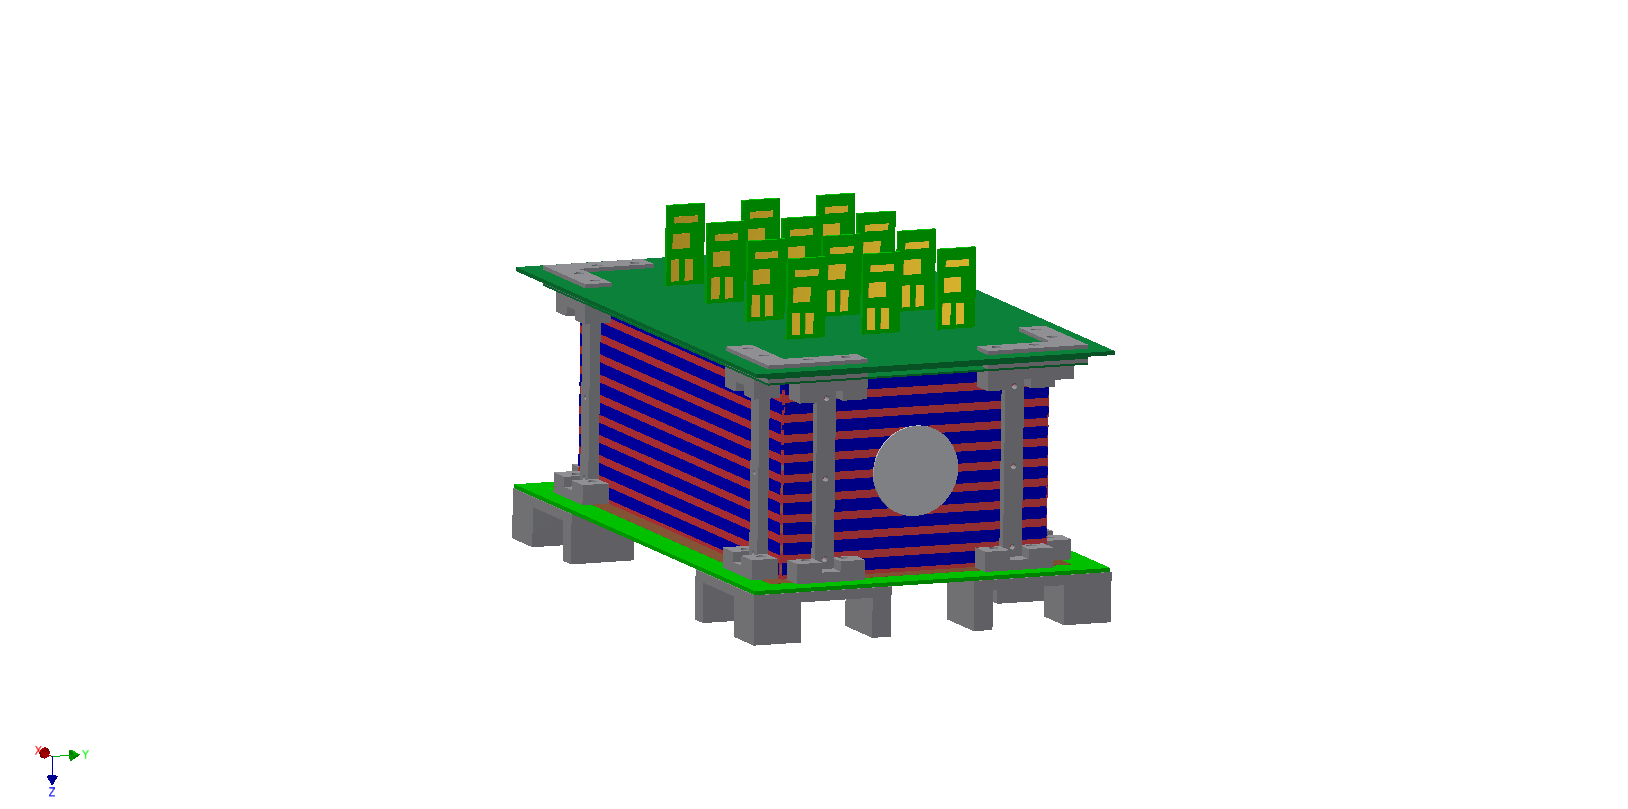
\includegraphics[width=0.8\textwidth]{./resource/CEE-TPC-Overview.png}
	\caption{TPC结构示意图:下部为阴极,上部为阳极,四周围以加有阶梯电压的
		金属条(红蓝的条状物);内部为灵敏区}
	\label{fig:det:TPC:Overview}
\end{figure}

CEE采用的TPC的结构如图\ref{fig:det:TPC:Overview}所示,上部为读出板。读出板
下方设置有一个大面积GEM膜,可以对漂移到TPC顶部的电子进行雪崩放大。读出板上
设置有12000个读出单元\cite{技术文档,Lyu:ConceptDesign},带电粒子
进入TPC后,其在灵敏区内产生的次级粒子将被竖直方向在读出板上投影位置的
读出单元感应到,从而由其在读出板上的投影给出其在水平平面内的位置信息;
我们已经知道次级粒子(电子)在TPC内近似以匀速运动,速度为
\SI{5}{\centi\meter/\micro\second},其飞行时间
(从电离到飞行至GEM被记录板感应到的飞行时间)被用于确定事件在竖直方向的位置。

在本框架中,这一过程被抽象为:首先将探测器按照读出板上的读出单元分成若干个小室,
每个小室对应一个读出单元的灵敏区;粒子进入TPC时,在每个小室内产生的总能量损失和
发生事件的位置与时间会被记录。这里与上述原理主要的区别是本框架内为了提高模拟效率,
只构建了TPC内的磁场,而暂时还没有构建TPC内的电场,也没有模拟电子真实的漂移过程
或在GEM上的雪崩放大;因此,我们假设电离产生的次级电子会在TPC内短时间内减速而
失去其初始动能(从而忽略减速过程中所受的电场作用),随后受到电场力作用匀速到达
GEM膜而被放大和被探测到;
%TODO:考虑复合
其中,目前本框架尚未考虑这两个过程中被复合而损失的电子,
因此本框架记录和存储的是所有终止在TPC内的电子的位置和时间信息。

事实上,由于TPC中所有次级电子最终都是匀速飞向记录板的,因此TPC并不对康普顿效应、
各种热效应等不产生次级电子的能量损失敏感,而是只对次级电子的产生敏感;因此,
本框架在完成TPC的数字化过程时,可以认为TPC的输出结果就是每个记录单元所应当
感应到的电子数目和触发该记录单元的时间。目前本框架在每个模拟事件结束时,
将这些电子归入设定好的小室,确定每个次级电子将会被哪个或哪些记录单元记录到;
最后输出每个记录单元所应当记录到的电子个数和触发时间。
%TODO:考虑死时间
这一过程中,本框架暂时没有考虑记录板的死时间问题,因此记录下来的是飞行到GEM膜
的总电子数目;
%TODO:Y坐标与时间的关系
尽管次级电子在TPC内匀速运动,但具体的竖直方向坐标与漂移时间的关系还需要实验
定标,本框架目前近似认为感应到信号所花的时间就是电子以一定的漂移速度
\SI{5}{\centi\meter/\micro\second}飞行到GEM膜的时间。

本框架的TPC记录器将模拟得到的数据存储在一个以各个电子的跟踪编号(TrackID)为
键值的字典对象中,为每个键值存储其最后一次被跟踪时的位置和时间;飞出TPC的
电子对应的记录将被清除,因为其将无法在TPC中受到电场作用而飞向GEM膜,从而不会
被TPC感应到;相反,在TPC外电离产生而飞入TPC的电子将会被记录。本框架的输出系统
会在每次事件结束时先输出各个次级电子的跟踪信息(编号、最后位置和时间),再输出
每个读出单元所应当读到的电子数目与触发时间。

\subsection{MRPC记录}\label{ssec:digi:MRPC}

CEE中使用的飞行时间探测器由多层MRPC阵列组成,各测量单元交错布置,以最大限度减小死区。
在第\ref{ssec:det:tof}节中已经提到,本框架分四层构建了这种基于MRPC的TOF探测器。
用于数字化时,本框架以第三层的每个MRPC单位作为记录的单位。数字化过程中,本框架
假设任何发生在灵敏区(不包括玻璃板这种非灵敏区)的有能量沉积的步骤都能够被MRPC
的记录板探测到,并立即在记录板的对应位置产生一个能够以$v=\frac23c$速度($c$为真空
光速)向两端的读出电子学传输的信号。

由于MRPC的子结构丰富,同时也由于本框架支持外部数据、而依照这种数据构建的MRPC结构
有一定的不确定性,因此本记录器在记录过程中将数据以运行时查询到的各个MRPC单元的
名称为键值存储在字典对象中,为每个MRPC单元存储了其几何信息,并分配了一个可变长度
的列表,用于存储其中发生的所有有效步骤的时间和位置信息。

本记录器会在任何步骤出现在MRPC灵敏区内时保存这一事件,取得其几何信息,并计算出
两端读出的时间,追加到在字典对象中为这个MRPC单元提供的不定长列表中。
随后,本记录器记录了每个MRPC每端读出时间的最小值,认为其为这一端实际
收到信号的时间;连同(有可能由于用户设置数据而发生改变的)几何信息输出到预定的
输出文件中。

\subsection{MWDC记录}\label{ssec:digi:MWDC}

在本框架中,MWDC系统实际上是一套位置灵敏探测器。本框架假设MWDC由均匀分布的三层灵敏层
组成,每层灵敏层上以固定距离平行设置了若干灵敏丝(阳极丝)。与TPC类似,本框架出于
效率考虑,没有实际几何构建阳极丝或阴极丝,也没有实际构建其产生的电场,忽略了电场
%TODO:考虑复合
对次级粒子产生过程的影响,也忽略了次级电子的复合;假设阳极丝能产生一个圆柱形的
灵敏区,任何进入该灵敏区的次级电子都将被该阳极丝俘获并进入漂移过程;本框架视这些
进入漂移的电子不再发生其他效应。也就是说,本框架将记录每个次级电子第一次进入灵敏区
时的状态。

与TPC记录器类似,MWDC记录器将模拟得到的数据存储在以各个电子的跟踪编号(TrackID)
为键值的字典对象中,但为每个电子存储的信息是其所触发的丝、触发时与丝的距离和
触发时间。本框架跟踪模拟中出现在MWDC内的所有次级电子,在每一步检查该电子是否出现在
任何一根灵敏丝的灵敏区内;只要存在这样的灵敏区,就在字典中为该电子创建记录,记录
其所触发的丝、与该丝的距离和当前时间。当字典中已经存在这样的触发信息后,记录器
就不会再响应该电子的任何步骤了:因为如上所述,该电子被假定进入了漂移过程,不会再
参与任何其他的事件。本框架的输出系统最后会输出所有被认为有效的触发信息,以用于进一步
分析。

与TPC不同,MWDC的漂移时间与漂移距离之间的关系是非线性的(例如,文献\cite{Yi:MWDC}
中处理CEE的MWDC漂移距离时使用五次多项式拟合),在本模拟的假设下需要使用实验标定
的数据才能从漂移距离计算出漂移时间,因此本框架暂时还没有对MWDC像TPC那样计算漂移终止
的时间,而是直接记录了漂移开始的时间和漂移距离,并预备在以后的处理中再进一步数字化。

\section{数据输出}

本框架目前在每个Event的末尾,通过调用各个记录器的输出函数,直接将已经记录到各个
记录器的存储数据库中的记录数据直接输出到纯文本文件,按照每个Event产生一个记录文件
的方式输出。本框架目前使用一个函数模板实现对这些数据的输出;需要分析较大量的模拟
数据时,可以替换这一模板,将数据录入到ROOT等分析框架的数据结构中。在本文第
\ref{chap:例子}章中会以一个模拟事件为例具体分析输出的结果。

\section{径迹重建的基本原理}

本框架的分析功能要求中,对粒子在各探测器,尤其是多丝正比室中的径迹的重建是一个
核心要求。TPC可以利用记录单元和漂移时间确定粒子的径迹,但MWDC需要利用多层丝符合
确定粒子穿过MWDC的位置。本节中将介绍本工作中分析模拟数据时考虑MWDC径迹重建问题的
方法。

本工作目前分析的主要为模拟数据,模拟过程中每个入射粒子产生的事件都是独立的,因此
本工作分析的过程中无需考虑不同入射粒子产生的假符合。对于每块MWDC探测器,可以有
以下情况:
\begin{enumerate}
	\item 如果其三层丝中只有一层触发,则无法判断粒子在XY方向的入射位置。
	\item 如果有两层触发,且每一层都只有一根丝,那么其交点可以近似视为入射点。
		如果有灵敏层有不止一根丝,那么可以取其平均位置视为触发的丝,寻找交点。
	\item 如果有三层触发,且每层触发的丝构成的等腰三角形较小(例如内部不存在
		任何其他的灵敏丝),那么可以将其重心视为入射点。
\end{enumerate}

如果同侧的三块MWDC探测器中有至少两块能找出有效的入射点,那么可以利用这些探测器
得到的入射点连成直线,以确定粒子的运动方向。

% }}}

\chapter{模拟样例与分析}\label{chap:例子}
% {{{ 模拟样例与分析

本章将介绍本框架输出的模拟事件及对这些输出结果进行分析的一般方法。

\section{样例条件}

本章预备分析的模拟事件为采用本框架按照CEE预想预设的几何和材料等参数进行的对单个
入射粒子的模拟,入射粒子位于TPC正后方(即Z轴负半轴上)\SI{800}{\milli\meter}处、
具有能量\SI{250}{\mega\eV/u},方向沿探测器系统的主轴(即Z轴正方向)。框架编译为
单线程运行模式,并启用Geant4提供的Qt 4界面和OpenGL支持;运行时将Geant4 OpenGL的
允许显示单元数增加到1000000,以显示所需的大量探测器单元与束流径迹。

\section{事件显示}

样例模拟事件在本框架中可以利用模拟数据立即得到如图\ref{fig:EventDisplay}的显示。
可以看到,主径迹穿过\TZ、TPC后向X轴正方向(左侧)偏转,掠过左侧的MWDC1、MWDC2、
MWDC3和eTOF1,最终到达ZDC。

\begin{figure}
	\centering
	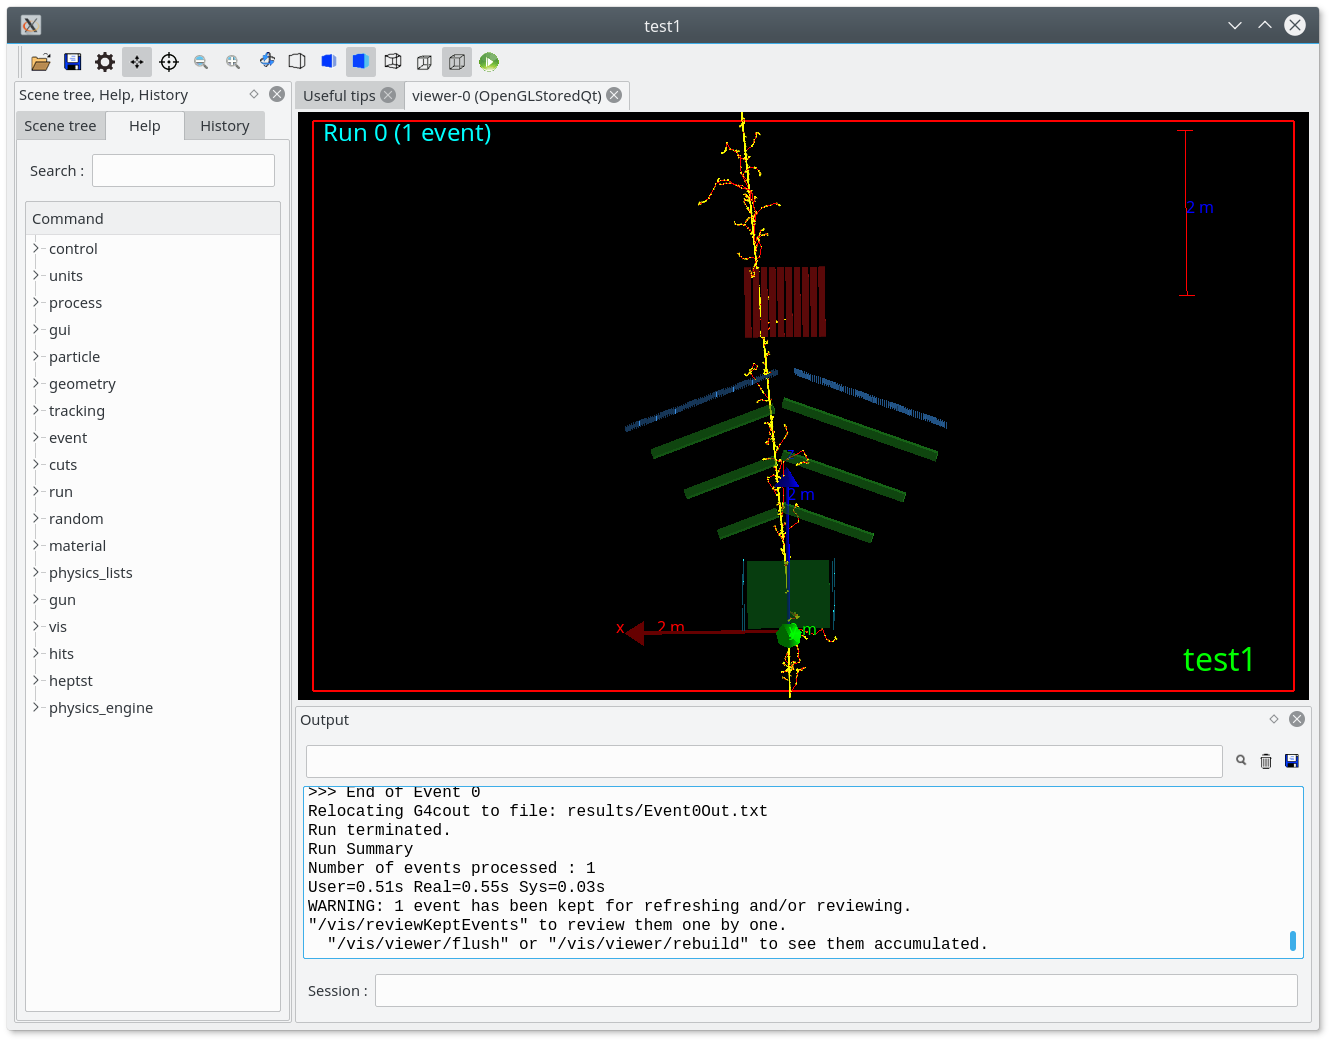
\includegraphics[width=0.7\textwidth]{./resource/EventDisplay.png}
	\caption{模拟事件显示}\label{fig:EventDisplay}
\end{figure}

\section{径迹测量}

径迹测量主要包括利用TPC和MWDC对粒子径迹的捕捉。

\subsection{TPC}

粒子在TPC中会发生偏转,过程中产生的次级电子将会漂移到记录板下方的GEM膜而被感应到。
本框架在输出过程中首先记录了每个次级粒子在TPC中进入漂移的位置和信息,随后为每个
记录单元计算了其最先记录到的感应信号的时间和飞到GEM膜被放大的次级电子的数目。
例如,样例事件首先可以得到类似附录\ref{chap:data}中代码\ref{data:TPC:Track}
的针对每个次级电子输出。

随后,本框架计算了每个
记录单元应当产生信号的强度和时间,并产生类似下面的输出(截取部分):

\begin{lstlisting}[caption={TPC Cells},firstnumber=3384,lastline=3387]
 >>> Cell:{1,-31} ElectronCount=7 SignalTime=7997.7270018879ns
 >>> Cell:{1,-30} ElectronCount=2 SignalTime=8000.3825638861ns
\end{lstlisting}

其中记录了每个记录单元(其灵敏区被称作小室,Cell)所应当感应到的次级电子的数目和
产生信号的时间。因此,本数据中TPC得到的输出结果可以绘制在图\ref{fig:result:TPC}中。

\begin{figure}
	\centering
	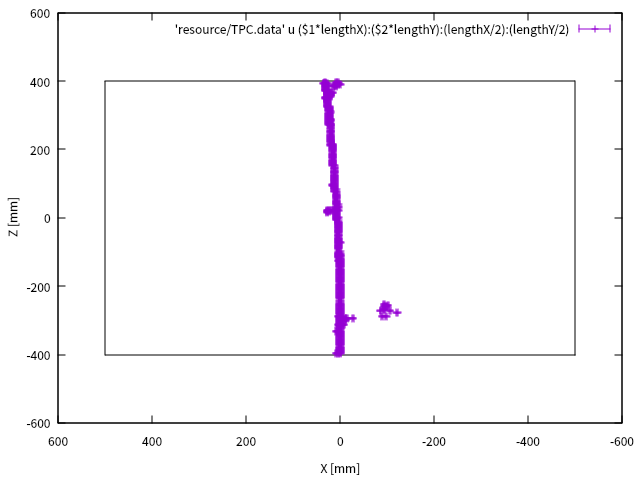
\includegraphics[width=0.7\textwidth]{./resource/TPC-result.png}
	\caption{TPC的输出结果,方框内为事件显示}\label{fig:result:TPC}
\end{figure}

据图\ref{fig:result:TPC}大致估计,离子向前运动\SI{800}{\milli\meter}后偏离了约
\SI{35}{\milli\meter};已知离子初始方向总是沿Z轴正方向的,那么离子在TPC内的曲率半径
$R$满足
\begin{equation}
(R-\SI{35}{\milli\meter})^2+(\SI{800}{\milli\meter})^2=R^2
\end{equation}
从而得到$R=\SI{9.16e3}{\milli\meter}$。代入到式\ref{eq:B}中,又有已知粒子带6个单位
正电荷、磁场磁感应强度为\SI{0.5}{\tesla}竖直向下,于是有
\begin{equation}
p=6\mathrm{e}\cdot\SI{0.5}{\tesla}\cdot\SI{9.16}{\meter}=\SI{27.48}{\eV\second
\meter^{-1}}=\SI{8.244e3}{\mega\eV/c}
\end{equation}
已知入射离子质量为\SI{12}{u},由相对论质量能量关系可以得到离子的初始动能$E$为:
\begin{equation}
\begin{aligned}
E &	=\sqrt{p^2c^2+m^2c^4}-mc^2\\
& 	=\sqrt{(\SI{8.244e3}{\mega\eV})^2+
		(\SI{1.1178e4}{\mega\eV})^2}-\SI{1.1178e4}{\mega\eV}\\
&	=\SI{2.711e3}{\mega\eV}
\end{aligned}\end{equation}
真实设定的入射离子能量为$\SI{250}{\mega\eV/u}=\SI{3e3}{\mega\eV}$,在同一数量级,
证明本框架较正确地模拟了TPC的功能。

\subsection{MWDC}

粒子经过MWDC时,可以在不同层的灵敏丝上产生不同的触发;利用各层丝上产生的触发,可以确定
粒子在MWDC不同层上经过的位置,从而确定粒子的径迹。

以示例数据为例,粒子扫过了MWDC1、MWDC2和MWDC3的边缘部分。其中,MWDC1的输出非常少:

\begin{lstlisting}[caption={MWDC1},firstnumber=3709,lastline=3710]
 >> TrackID=1833 StepID=12 ZLayer:0 WireNumber:-98 Distance=0.29491490749932mm kinectEnergy=0.10643500624019MeV Time=12.696963509901ns
 >> TrackID=9014 StepID=1 ZLayer:0 WireNumber:-98 Distance=0.29491490749932mm kinectEnergy=0.0039304610219273MeV Time=12.696963509901ns
\end{lstlisting}

这意味着粒子在X丝上只触发了一根-98号丝;这样并不能用于获得有效的轨迹。
而MWDC2得到的数据较多:

\begin{lstlisting}[caption={MWDC2},firstnumber=3760,lastline=3768]
 >> TrackID=2217 StepID=27 ZLayer:0 WireNumber:-280 Distance=0.79975751948989mm kinectEnergy=0.14046723287468MeV Time=17.349570175722ns
 >> TrackID=2537 StepID=1 ZLayer:0 WireNumber:-284 Distance=0.97771842475946mm kinectEnergy=0.0027493962453946MeV Time=15.453939879902ns
 >> TrackID=2568 StepID=1 ZLayer:1 WireNumber:-251 Distance=0.71580328112503mm kinectEnergy=0.001265401440291MeV Time=15.673162361ns
 >> TrackID=2569 StepID=1 ZLayer:1 WireNumber:-251 Distance=0.087115268746103mm kinectEnergy=0.0013009064838575MeV Time=15.677249124466ns
 >> TrackID=8861 StepID=1 ZLayer:0 WireNumber:-280 Distance=0.79975751948989mm kinectEnergy=0.0021034125376979MeV Time=17.349570175722ns
\end{lstlisting}

这意味着粒子分别触发了在X丝(编号为0)上编号为-280、-284和U丝(编号为1)上-251的丝
(负编号意味着在x方向上位于中间丝的右侧,正编号意味着左侧)。考虑到已知构建的MWDC2
的尺寸为$\SI{1171.4}{\milli\meter}\times\SI{999.8}{\milli\meter}$,而丝间距设定为
\SI{2}{\milli\meter},可以画出触发丝的示意图,如图\ref{fig:result:MWDC2}所示。

%粒子在MWDC3产生的事件更多:
%
%\begin{lstlisting}[caption={MWDC3},firstnumber=4052,lastline=4060]
% >> TrackID=2989 StepID=1 ZLayer:0 WireNumber:-367 Distance=0.82537430623022mm kinectEnergy=0.0017753140284645MeV Time=18.838334119299ns
% >> TrackID=2990 StepID=1 ZLayer:0 WireNumber:-367 Distance=0.58646172968141mm kinectEnergy=0.010074419957495MeV Time=18.841695213327ns
% >> TrackID=2991 StepID=1 ZLayer:0 WireNumber:-367 Distance=0.84791551639636mm kinectEnergy=0.001373249129488MeV Time=18.844855089962ns
% >> TrackID=3025 StepID=1 ZLayer:1 WireNumber:-324 Distance=0.98140871087136mm kinectEnergy=0.0013782070403012MeV Time=19.064825348212ns
% >> TrackID=3026 StepID=1 ZLayer:1 WireNumber:-324 Distance=0.95746977018064mm kinectEnergy=0.0012234780977097MeV Time=19.064986983029ns
% >> TrackID=3027 StepID=1 ZLayer:1 WireNumber:-324 Distance=0.89706618755126mm kinectEnergy=0.0030624322736415MeV Time=19.065404939646ns
% >> TrackID=3028 StepID=1 ZLayer:1 WireNumber:-324 Distance=0.56193634694886mm kinectEnergy=0.0020104794779073MeV Time=19.069155255952ns
% >> TrackID=3029 StepID=1 ZLayer:1 WireNumber:-324 Distance=0.5618470987962mm kinectEnergy=0.0021834659212389MeV Time=19.069172009923ns
% >> TrackID=3059 StepID=1 ZLayer:2 WireNumber:-327 Distance=0.87383127574681mm kinectEnergy=0.0014415503628428MeV Time=19.294719364388ns
%\end{lstlisting}
%
%这意味着粒子在X、U和V(编号为2)丝上各触发了一根丝,分别为编号-367、-324与-327。MWDC3
%设定的尺寸为$\SI{1582.9}{\milli\meter}\times\SI{999.8}{\milli\meter}$,而丝间距仍为
%\SI{2}{\milli\meter},可以画出如图\ref{fig:result:MWDC3}所示的示意图。
粒子在MWDC3上触发的事件反而较少:

\begin{lstlisting}[caption={MWDC3},firstnumber=4213,lastline=4215]
 >> TrackID=3099 StepID=1 ZLayer:0 WireNumber:-365 Distance=0.84163380144656mm kinectEnergy=0.0010520273465741MeV Time=18.835926733374ns
 >> TrackID=3100 StepID=1 ZLayer:0 WireNumber:-365 Distance=0.241168533277mm kinectEnergy=0.0017973460812635MeV Time=18.841395097067ns
 >> TrackID=3135 StepID=1 ZLayer:1 WireNumber:-321 Distance=0.76864959392221mm kinectEnergy=0.0014821410169985MeV Time=19.0639128482ns
\end{lstlisting}

这意味着粒子在X和U上各触发了一根丝,分别为编号-321和-365。MWDC3
设定的尺寸为$\SI{1582.9}{\milli\meter}\times\SI{999.8}{\milli\meter}$,而丝间距仍为
\SI{2}{\milli\meter},可以画出如图\ref{fig:result:MWDC3}所示的示意图。

\begin{figure}
	\centering
	\begin{subfigure}[c]{0.3\linewidth}
		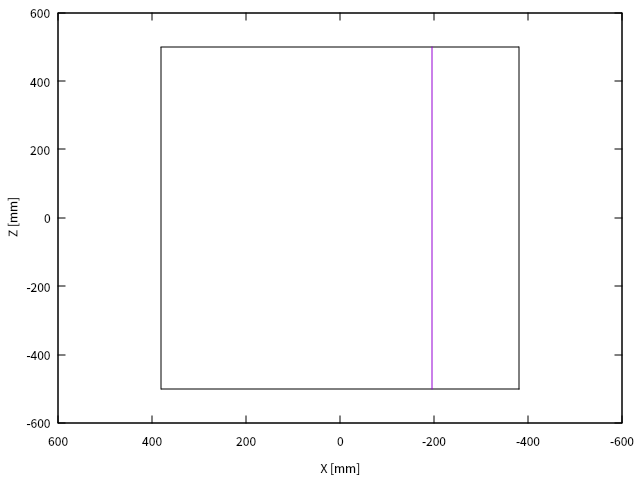
\includegraphics[width=\textwidth]{./resource/MWDC1-result.png}
		\subcaption{MWDC1}\label{fig:result:MWDC1}
	\end{subfigure}
	\begin{subfigure}[c]{0.3\linewidth}
		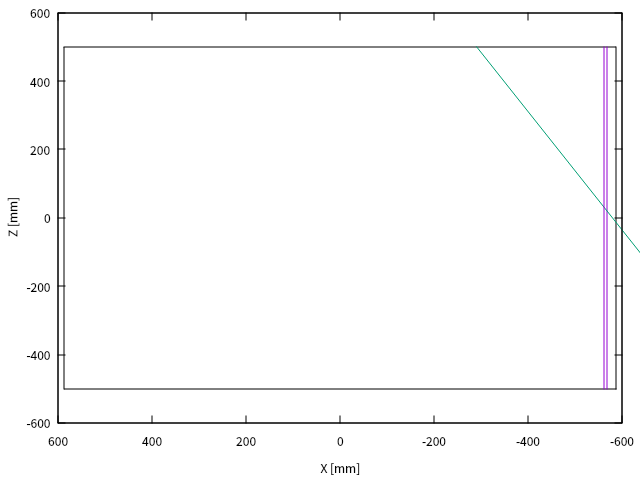
\includegraphics[width=\textwidth]{./resource/MWDC2-result.png}
		\subcaption{MWDC2}\label{fig:result:MWDC2}
	\end{subfigure}
	\begin{subfigure}[c]{0.3\linewidth}
		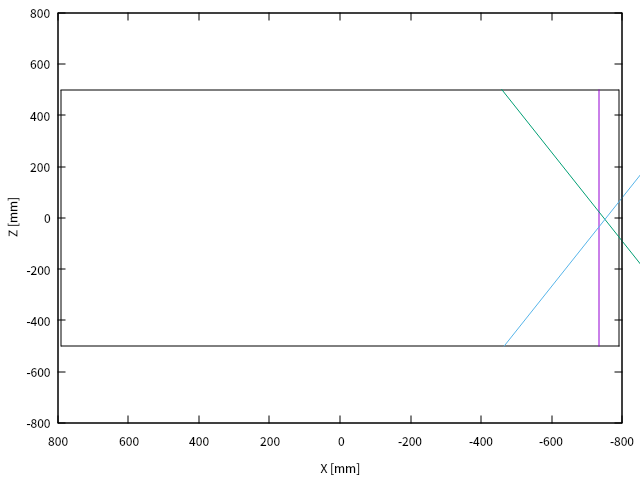
\includegraphics[width=\textwidth]{./resource/MWDC3-result.png}
		\subcaption{MWDC3}\label{fig:result:MWDC3}
	\end{subfigure}
	\caption{MWDC的触发丝示意图。其中黑框为MWDC的灵敏区,紫色线为X丝,
		绿色线为U丝,青色线为V丝。}
	\label{fig:result:MWDC}
\end{figure}

本示例事件中MWDC系统没能得到足够实现重建的数据。
在图\ref{fig:MWDC:EventDisplay}中我们其实可以看出,事实上本模拟事件中主粒子并没有真的
穿过MWDC,因此本模拟事件中得到很少的数据点也是正常的。

\begin{figure}
	\centering
	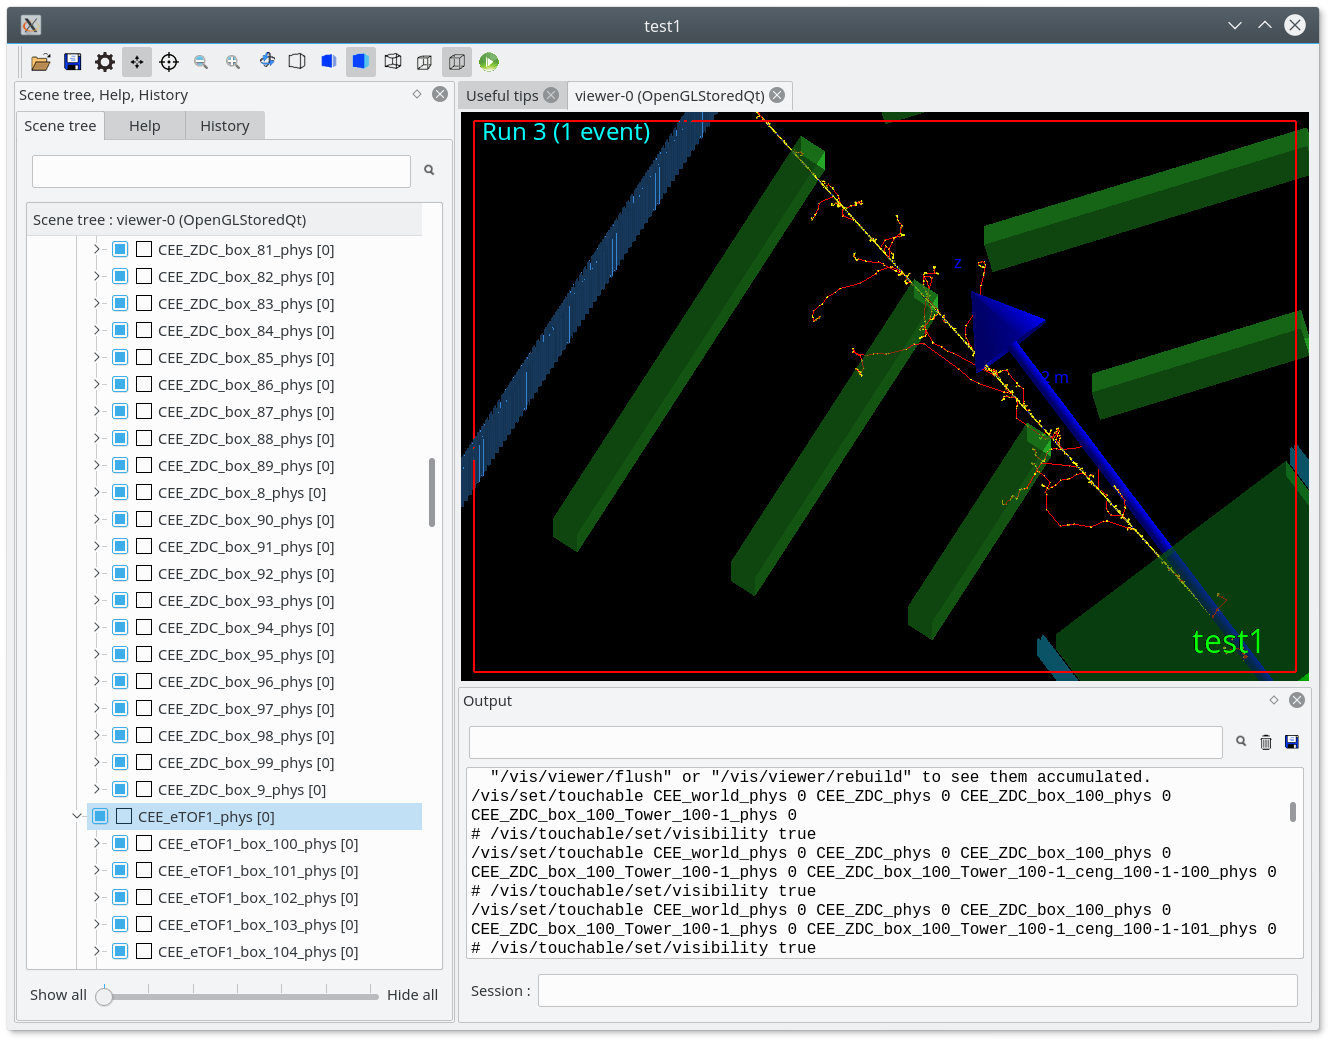
\includegraphics[width=0.8\textwidth]{./resource/MWDC-EventDisplay.png}
	\caption{粒子通过MWDC的示意图}
	\label{fig:MWDC:EventDisplay}
\end{figure}

\section{零度角量能}

零度角量能器的每个Tower都可以给出其灵敏区得到的能量,并分别输出。没有记录到任何事件
的Tower不会输出,以此优化输出的结果。例如,对于示例事件,共有6个Tower记录到了能量
沉积(从而会有输出);这些Tower在探测器内的位置大致如图\ref{fig:result:ZDC:Display}
所示。

\begin{figure}
	\centering
	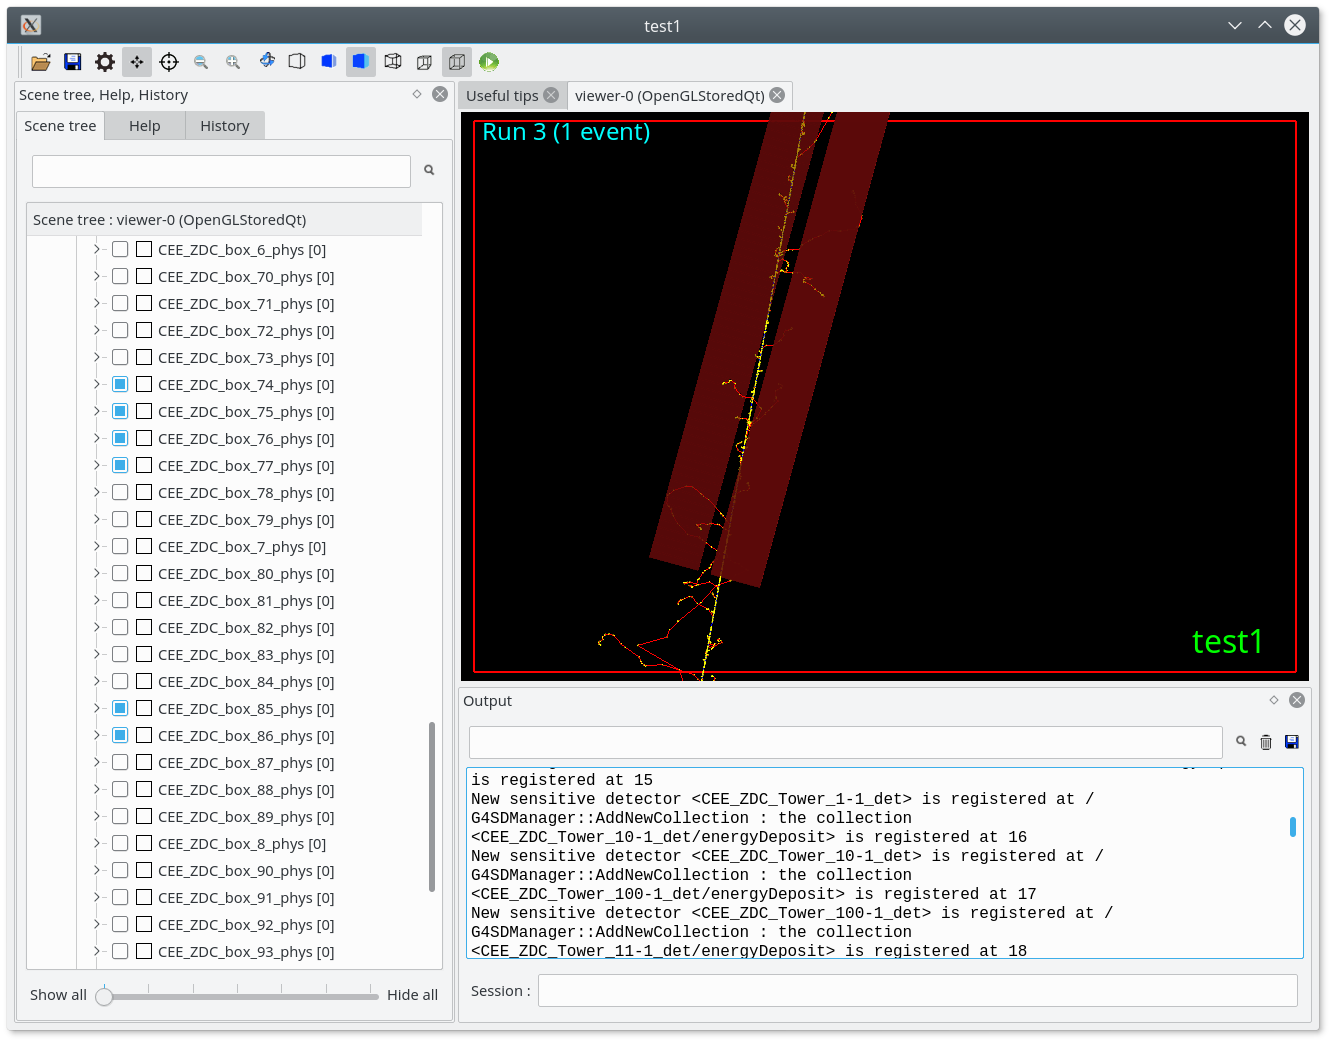
\includegraphics[width=0.7\textwidth]{./resource/ZDC-Display.png}
	\caption{产生闪烁信号的ZDC Tower}\label{fig:result:ZDC:Display}
\end{figure}

\section{飞行时间测量}

示例事件中实际上主粒子只经过了eTOF1,并在eTOF1中留下了触发信号。发生触发的MRPC
得到了类似附录\ref{chap:data}中代码\ref{data:MRPC}的输出。省略各跟踪的具体数据的
结果如代码\ref{data:MRPC:short}所示。
\begin{lstlisting}[caption={eTOF1-MRPC简略版,其中所有size均为半长度},
	numbers=none,label={data:MRPC:short}]
 >>> MRPC: CEE_eTOF1_box_70_MRPC_70-1_phys
   > sizeX=3mm sizeY=1000mm sizeZ=2.25mm 
 >>> Time=23.232219654236ns ATime=27.729055198431ns BTime=28.726130467889ns
 >>> MRPC: CEE_eTOF1_box_70_MRPC_70-2_phys
   > sizeX=3mm sizeY=1000mm sizeZ=2.25mm 
 >>> Time=23.159832890205ns ATime=27.622659457019ns BTime=28.703491862312ns
 >>> MRPC: CEE_eTOF1_box_74_MRPC_74-2_phys
   > sizeX=3mm sizeY=1000mm sizeZ=2.25mm 
 >>> Time=21.38632894461ns ATime=26.39209786613ns BTime=26.387482879035ns
 >>> MRPC: CEE_eTOF1_box_75_MRPC_75-1_phys
   > sizeX=3mm sizeY=1000mm sizeZ=2.25mm 
 >>> Time=21.389191097435ns ATime=26.299618590779ns BTime=26.485686460035ns
 >>> MRPC: CEE_eTOF1_box_85_MRPC_85-1_phys
   > sizeX=3mm sizeY=1000mm sizeZ=2.25mm 
 >>> Time=21.277339016766ns ATime=26.240804097681ns BTime=26.320796791796ns
\end{lstlisting}

其中,ATime为信号到达上端的时间,BTime为信号到达下端的时间。利用已知的信号传播速度
$v=\frac23c$($c$为真空光速)和已知的Y方向尺寸,可以从两个信号时间计算出触发信号的
实际时间。例如,对于编号为85-1的MRPC,实际时间可以计算为
\begin{equation}
\frac{t_{\text{ATime}}+t_{\text{BTime}} }{2}-\frac{d_{\text{sizeY}} }{v}
	=\SI{21.28}{\nano\second}
\end{equation}
(直接记录的值为\SI{21.278}{\nano\second})
也可以由这两个时间计算触发信号的位置:两端时间差相当于2倍于Y方向坐标值除以速度,
于是有
\begin{equation}
\frac{t_{\text{ATime}}-t_{\text{BTime}} }{2}=-\frac{y}{v}=\SI{-0.08}{\nano\second}
\end{equation}
得到$y=\SI{8}{\milli\meter}$。事实上,85-1模拟测量的详细数据如代码\ref{data:MRPC:85-1}
可以看到,Y方向坐标确实在\SI{8}{\milli\meter}左右:
\begin{lstlisting}[caption={eTOF1-MRPC-85-1},label={data:MRPC:85-1},firstnumber=4449,lastline=4453]
 >>> MRPC: CEE_eTOF1_box_85_MRPC_85-1_phys
   > sizeX=3mm sizeY=1000mm sizeZ=2.25mm 
 >>> Time=21.277339016766ns ATime=26.240804097681ns BTime=26.320796791796ns
 >>>> tID=3516 sID=4 pX=-2.154416372819mm pY=7.9937354635887mm pZ=-2.25mm Time=21.277339016766ns ATime=26.240804097681ns BTime=26.320796791796ns
 >>>> tID=3516 sID=6 pX=-2.6107045517469mm pY=8.3243743706931mm pZ=-1.5499999999997mm Time=21.281163615032ns ATime=26.242974356929ns BTime=26.32627572908ns
\end{lstlisting}

实际实验中,这一时间还将受到电子学延迟等的影响,因此用于实验分析时需要使用标定好
的时间信息。目前本框架的模拟忽略了这些因素的影响。

% }}}

\chapter*{结论}\addcontentsline{toc}{chapter}{结论}
% {{{ 结论
本工作中,基于HIRFL-CSR外靶实验(CEE)的设计方案,构建了基于Geant4的实验模拟框架,
并基于现有的径迹重建方法和模拟得到的数据考虑了重建的方案,通过对模拟数据的分析评价
了模拟框架的构建。其中,本框架的核心和创造性工作主要集中在于第\ref{sec:digi}节讨论
的对时间投影室(TPC)、多丝漂移室(MWDC)和多气隙电阻板室(MRPC)的数字化方案与实现。
本框架假定TPC对失去初始能量后进入匀速漂移的次级电子敏感,构建了针对次级电子的最后
一个跟踪步骤的TPC记录器,并计算次级粒子的漂移时间,将记录的各电子数据归入TPC的
各记录单元,得到了模拟事件中TPC记录板上各记录单元得到信号的强度和触发时间;假定
MWDC对进入任何灵敏丝的灵敏范围的次级电子敏感,构建了针对次级电子第一个接触灵敏区
的跟踪步骤的MWDC记录器,得到了MWDC上所触发丝的编号和漂移时间;假定MRPC对灵敏区内
发生的任何产生能量沉积的事件敏感,记录了其触发的位置和时间,并计算得到了模拟事件中
MRPC两端读出时两端各自的触发时间。本工作中构建的这三个记录器实现了对TPC、MWDC和
MRPC的数字化,可以广泛地用于对与CEE采用构型相似的这三种探测器的模拟分析。

本工作开展时间不长,在完成的工作范围内仍然存在若干需要进一步讨论的问题。例如,
探测器的死时间问题尚未讨论,次级电子的复合等问题还未列入考虑范围,CEE中部分探测器
(如\TZ)的设计方案有较大变动等。由于CEE是一个正在设计和准备过程中的实验,本工作
在完成基本构建后仍将持续进行,针对CEE需要讨论的各种新问题对模拟框架进行持续改进,
并针对CEE的分析要求继续构建更多的分析功能。

% }}}

% 致谢
% !Mode:: "TeX:UTF-8"
\chapter*{致谢}
\addcontentsline{toc}{chapter}{致谢}
本文是在清华大学物理系的实验核物理研究组的指导下完成的。其中,径迹重建的方法源于课题组
博士生吕黎明的实验分析课题;几何构建和数字化等工作是和同为研究组成员的本科生秦智同学合
作完成的。
\cleardoublepage

% 参考文献
%\include{data/reference}
\printbibliography[heading=bibintoc,title={参考文献}]

% 附录
\appendix
\chapter{源代码仓库}\label{chap:repo}
% {{{ 源代码仓库
本工作中构建的模拟与分析框架的源代码仓库位于
\url{https://github.com/qinq-net/CEE.git}。编译和安装本框架需要首先保证能够通过
库搜索路径找到一个可用的、支持Qt及OpenGL功能的Geant4框架。本工作中在Linux系统中安装了
CLHEP 2.3.3.1和Qt 4.8.7,打开了Geant4的Qt4、GDML和OpenGL支持,并关闭了多线程支持,
亦即采用了以下参数配置Geant4的cmake:

\begin{lstlisting}[caption={Geant4 编译选项}]
GEANT4_USE_SYSTEM_CLHEP=ON
GEANT4_BUILD_MULTITHREADED=OFF
GEANT4_USE_GDML=ON
GEANT4_USE_OPENGL_X11=ON
GEANT4_USE_QT=ON
GEANT4_FORCE_QT4=ON
\end{lstlisting}

本框架主要实现的类如下所示。

\begin{lstlisting}[caption={主要实现的类}]
T1DetectorConstruction	# 探测器构建与灵敏探测器分配
T1TPC			# TPC构建
T1TPCDigi		# TPC的灵敏探测器
CEEPSTPCScorer		# TPC的记录器
T1MWDC 			# MWDC构建
T1MWDCDigi		# MWDC的灵敏探测器
CEEPSMWDCScorer		# MWDC的记录器
T1T0			# \TZ构建
T1iTOF 			# iTOF构建
T1eTOF 			# eTOF构建
T1MRPCDigi 		# TOF的MRPC灵敏探测器
CEEPSMRPCScorer		# TOF的MRPC的记录器
\end{lstlisting}
% }}}

\chapter{示例数据}\label{chap:data}
% {{{ 示例数据

示例数据可以在
{\do{\/}\do{-}
\url{https://github.com/qinq-net/BUAAthesis/blob/QIN/resource/EventExampleOut.txt}
}
找到。以下是部分在文中提及的较长数据。

\section{TPC Tracks}\label{sec:data:TPC:Track}

以下的代码\ref{data:TPC:Track}
是TPC记录的跟踪数据的截取部分的样例。其中每行记录了一个在TPC内进入漂移的次级电子
最后所在的位置和时间;XZ方向(平行于记录板)的位置记录的是其漂移最终将产生信号的
记录单元的编号。
\begin{lstlisting}[caption={TPC Tracks},label={data:TPC:Track},firstnumber=2650,lastline=2657]
 >> TrackID=995 CellXZ={1,-31} positionY=0.42669649210073mm Time=6.2609317299298ns
 >> TrackID=996 CellXZ={0,-31} positionY=-1.2316577587387mm Time=6.3574588373838ns
 >> TrackID=997 CellXZ={1,-31} positionY=0.29267780410593mm Time=6.2579124256321ns
 >> TrackID=998 CellXZ={1,-31} positionY=0.29271473410068mm Time=6.2582254078705ns
 >> TrackID=999 CellXZ={1,-30} positionY=0.29312751180922mm Time=6.2616937324113ns
 >> TrackID=1000 CellXZ={1,-30} positionY=0.29456414464476mm Time=6.273846779001ns
 >> TrackID=1001 CellXZ={0,-30} positionY=-48.618680814943mm Time=7.226464863741ns
 >> TrackID=1002 CellXZ={1,-28} positionY=0.29686598769096mm Time=6.2947223883586ns
\end{lstlisting}
%{./resource/EventExampleOut.txt}

\section{MRPC (eTOF1)}\label{sec:data:MRPC}
以下的代码\ref{data:MRPC}
是MRPC(eTOF1)的示例数据。其中记录了每个MRPC单元的时间信息,以及每个单元内
追踪到的每个有关次级电子的有关信息。所有标注size的均为半长度;ATime指沿Y正方向
记录信号的时间,BTime指沿负方向记录的时间,pX、pY、pZ为事件相对灵敏区中心的坐标,
tID为跟踪编号(次级电子的编号),sID为步骤编号(每个电子被记录时在Geant4中经过
了多少步跟踪)。
\begin{lstlisting}[caption={eTOF1:MRPC},label={data:MRPC},firstnumber=4397,lastline=4453]
>> MultiFunctionalDet  CEE_6T1eTOF1_det
>> PrimitiveScorer MRPCScorer
>> Number of copies 1
>> Direction:Y
 >  copy no.: 0
 >  Number of entries 5
 >>> MRPC: CEE_eTOF1_box_70_MRPC_70-1_phys
   > sizeX=3mm sizeY=1000mm sizeZ=2.25mm 
 >>> Time=23.232219654236ns ATime=27.729055198431ns BTime=28.726130467889ns
 >>>> tID=3516 sID=46 pX=-0.65058607962794mm pY=98.022017905248mm pZ=2.0999999999999mm Time=23.232219654236ns ATime=27.745231696528ns BTime=28.726130467889ns
 >>>> tID=8530 sID=24 pX=-2.6389353759629mm pY=107.13286272149mm pZ=2.25mm Time=23.261628916754ns ATime=27.729055198431ns BTime=28.801125491022ns
 >>>> tID=8530 sID=25 pX=-2.5958838875816mm pY=107.181624516mm pZ=2.1582458112139mm Time=23.264212011758ns ATime=27.731394315678ns BTime=28.803952563784ns
 >>>> tID=8530 sID=31 pX=-2.8025229389467mm pY=107.31999234494mm pZ=2.0999999999999mm Time=23.2761427419ns ATime=27.742632727724ns BTime=28.81657561202ns
 >>>> tID=8530 sID=32 pX=-2.768969355109mm pY=107.34106952607mm pZ=2.1027356555733mm Time=23.277701027931ns ATime=27.744085554892ns BTime=28.818239356914ns
 >>> MRPC: CEE_eTOF1_box_70_MRPC_70-2_phys
   > sizeX=3mm sizeY=1000mm sizeZ=2.25mm 
 >>> Time=23.159832890205ns ATime=27.622659457019ns BTime=28.703491862312ns
 >>>> tID=3516 sID=43 pX=2.4980398831841mm pY=107.86636253925mm pZ=2.25mm Time=23.160325249999ns ATime=27.62408149363ns BTime=28.703491862312ns
 >>>> tID=8530 sID=2 pX=2.4301012778606mm pY=108.05216927146mm pZ=2.25mm Time=23.159832890205ns ATime=27.622659457019ns BTime=28.703929179336ns
 >>> MRPC: CEE_eTOF1_box_74_MRPC_74-2_phys
   > sizeX=3mm sizeY=1000mm sizeZ=2.25mm 
 >>> Time=21.38632894461ns ATime=26.39209786613ns BTime=26.387482879035ns
 >>>> tID=1 sID=4139 pX=-1.0818917804255mm pY=-0.46117944167399mm pZ=-2.25mm Time=21.38632894461ns ATime=26.39209786613ns BTime=26.387482879035ns
 >>>> tID=1 sID=4142 pX=-1.2698106859326mm pY=-0.46165504931311mm pZ=-1.5499999999997mm Time=21.390288340233ns ATime=26.396059641437ns BTime=26.391439894973ns
 >>>> tID=1 sID=4143 pX=-1.3265208868776mm pY=-0.46179907778646mm pZ=-1.3387570644636mm Time=21.391483191589ns ATime=26.397255213435ns BTime=26.392634025689ns
 >>>> tID=1 sID=4145 pX=-1.4644420275589mm pY=-0.4621519609717mm pZ=-0.82499999999982mm Time=21.394389149811ns ATime=26.400162937294ns BTime=26.395538218273ns
 >>>> tID=1 sID=4146 pX=-1.5119192492919mm pY=-0.46227099766786mm pZ=-0.64815077929597mm Time=21.395389462042ns ATime=26.40116384512ns BTime=26.396537934908ns
 >>>> tID=1 sID=4149 pX=-1.6389447059718mm pY=-0.46260273137077mm pZ=-0.17499999999973mm Time=21.398065785279ns ATime=26.403841828174ns BTime=26.399212598328ns
 >>>> tID=1 sID=4151 pX=-1.8403064704808mm pY=-0.46312361480218mm pZ=0.57499999999982mm Time=21.402308094122ns ATime=26.408086743238ns BTime=26.403452300952ns
 >>>> tID=1 sID=4153 pX=-2.0148085007131mm pY=-0.4635467815832mm pZ=1.2249999999999mm Time=21.405984749041ns ATime=26.411765515455ns BTime=26.407126838571ns
 >>>> tID=1 sID=4155 pX=-2.2497160231134mm pY=-0.46411398762958mm pZ=2.0999999999999mm Time=21.410934099272ns ATime=26.416717703679ns BTime=26.412073350808ns
 >>>> tID=3549 sID=7 pX=-2.6961443413721mm pY=-0.84156360466936mm pZ=2.25mm Time=21.4271875672ns ATime=26.434859726207ns BTime=26.426438264137ns
 >>>> tID=3549 sID=8 pX=-2.7339948315214mm pY=-0.82203666973835mm pZ=2.2018705711821mm Time=21.429182700825ns ATime=26.436757157567ns BTime=26.428531100028ns
 >>>> tID=3549 sID=9 pX=-2.7879444376543mm pY=-0.82871568477737mm pZ=2.1844554933036mm Time=21.431159317671ns ATime=26.438767192606ns BTime=26.430474298679ns
 >>>> tID=3547 sID=1 pX=-1.5119192492919mm pY=-0.46227099766786mm pZ=-0.64815077929597mm Time=21.395389462042ns ATime=26.40116384512ns BTime=26.396537934908ns
 >>>> tID=3547 sID=3 pX=-1.6109878892759mm pY=0.35587952352952mm pZ=-0.17499999999973mm Time=21.400946487778ns ATime=26.402627286282ns BTime=26.40618854522ns
 >>>> tID=3547 sID=5 pX=-1.7461507440819mm pY=1.6512353590846mm pZ=0.57499999999982mm Time=21.409768900821ns ATime=26.404968436366ns BTime=26.421492221221ns
 >>>> tID=3547 sID=7 pX=-1.8724403209965mm pY=2.5582768952308mm pZ=1.2249999999999mm Time=21.416368329201ns ATime=26.407029517406ns BTime=26.432629996941ns
 >>>> tID=3547 sID=9 pX=-1.9849118157607mm pY=3.9633714689195mm pZ=2.0999999999999mm Time=21.426144164423ns ATime=26.409775016126ns BTime=26.449436168665ns
 >>>> tID=3546 sID=1 pX=-1.3265208868776mm pY=-0.46179907778646mm pZ=-1.3387570644636mm Time=21.391483191589ns ATime=26.397255213435ns BTime=26.392634025689ns
 >>>> tID=3544 sID=3 pX=-1.0755909817432mm pY=-0.37487647317133mm pZ=-2.2500000000005mm Time=21.389177840605ns ATime=26.394514948551ns BTime=26.390763588603ns
 >>>> tID=3544 sID=4 pX=-1.0856452082846mm pY=-0.32941961749369mm pZ=-2.2087539711483mm Time=21.391179397271ns ATime=26.396289063593ns BTime=26.392992586894ns
 >>> MRPC: CEE_eTOF1_box_75_MRPC_75-1_phys
   > sizeX=3mm sizeY=1000mm sizeZ=2.25mm 
 >>> Time=21.389191097435ns ATime=26.299618590779ns BTime=26.485686460035ns
 >>>> tID=3516 sID=11 pX=-0.4099040229919mm pY=18.593914626368mm pZ=-2.25mm Time=21.389191097435ns ATime=26.299618590779ns BTime=26.485686460035ns
 >>>> tID=3516 sID=13 pX=-0.82740797236124mm pY=19.066229334085mm pZ=-1.5500000000002mm Time=21.393220518132ns ATime=26.301284803054ns BTime=26.492079089154ns
 >>>> tID=3516 sID=15 pX=-1.2250612426719mm pY=19.569985966183mm pZ=-0.82499999999982mm Time=21.397362655399ns ATime=26.302906413444ns BTime=26.498741753299ns
 >>>> tID=3516 sID=17 pX=-1.5697601280742mm pY=20.01468751464mm pZ=-0.17500000000018mm Time=21.401041072686ns ATime=26.304359783686ns BTime=26.504645217631ns
 >>>> tID=3516 sID=19 pX=-1.9753022860094mm pY=20.5490818585mm pZ=0.57499999999982mm Time=21.405346825696ns ATime=26.305991715209ns BTime=26.511624792127ns
 >>>> tID=3516 sID=21 pX=-2.319985779691mm pY=21.002418569207mm pZ=1.2249999999999mm Time=21.409044738455ns ATime=26.307421375222ns BTime=26.517590957632ns
 >>>> tID=3516 sID=23 pX=-2.7788220459133mm pY=21.597965650609mm pZ=2.1000000000004mm Time=21.41398174057ns ATime=26.309378580486ns BTime=26.525507756597ns
 >>> MRPC: CEE_eTOF1_box_85_MRPC_85-1_phys
   > sizeX=3mm sizeY=1000mm sizeZ=2.25mm 
 >>> Time=21.277339016766ns ATime=26.240804097681ns BTime=26.320796791796ns
 >>>> tID=3516 sID=4 pX=-2.154416372819mm pY=7.9937354635887mm pZ=-2.25mm Time=21.277339016766ns ATime=26.240804097681ns BTime=26.320796791796ns
 >>>> tID=3516 sID=6 pX=-2.6107045517469mm pY=8.3243743706931mm pZ=-1.5499999999997mm Time=21.281163615032ns ATime=26.242974356929ns BTime=26.32627572908ns
\end{lstlisting}
% }}}

%\include{data/appendix1-faq}
%\include{data/appendix2-contactus}
\end{document}
